\subsection{Construction de \texorpdfstring{$\mathbb{N}$}{N}}
\label{sub:constN}

\subsubsection{Définition}

L'ensemble des entiers naturels, noté $\mathbb{N}$\sindex[isy]{$\mathbb{N}$}, est défini de la manière suivante. 
Notons $\mathrm{Cl}$ le prédicat à un paramètre libre défini par :
\begin{equation*}
    \mathrm{Cl}(A): (\emptyset \in A) \wedge (\forall a \, (a \in A \Rightarrow a \cup \lbrace a \rbrace \in A)). 
\end{equation*}
D'après l'axiome de l'infini, il existe un ensemble $A$ tel que $\mathrm{Cl}(A)$ est vrai.
Soit $\mathrm{Ent}$ le prédicat à un paramètre libre défini par : 
\begin{equation*}
    \mathrm{Ent}(x): \forall A \, (\mathrm{Cl}(A) \Rightarrow x \in A). 
\end{equation*}
Soit $I$ un ensemble tel que $\mathrm{Cl}(I)$ est vrai. 
L'ensemble $\mathbb{N}$ est défini par : 
\begin{equation*}
     \mathbb{N} = \lbrace x \in I \vert \mathrm{Ent}(x) \rbrace. 
\end{equation*}
Notons que cette définition ne dépend pas du choix de $I$. 
Notons aussi que $\emptyset \in \mathbb{N}$ et $\forall n \, n \in \mathbb{N} \Rightarrow n \cup \lbrace n \rbrace \in \mathbb{N}$.

\medskip

\noindent\textbf{Démonstration :}

\begin{itemize}[nosep]
    \item Montrons d'abord que $\emptyset \in \mathbb{N}$. 
        Puisque $\mathrm{Cl}(I)$ est vrai, $\emptyset \in I$.
        Soit $A$ un ensemble tel que $\mathrm{Cl}(A)$ est vrai.
        Alors, $\emptyset \in A$.
        Donc, $\mathrm{Ent}(\emptyset)$ est vrai. 
        On a donc $\emptyset \in I \wedge \mathrm{Ent}(\emptyset)$. 
        Donc, $\emptyset \in \mathbb{N}$.
    \item Soit $n$ un élément de $\mathbb{N}$. 
        Alors, $n \in I$.
        Puisque $\mathrm{Cl}(I)$ est vrai, on en déduit que $n \cup \lbrace n \rbrace \in I$.
        Soit $A$ un ensemble tel que $\mathrm{Cl}(A)$ est vrai.
        Puisque $\mathrm{Ent}(n)$ est vrai, $n \in A$.
        Alors, puisque $\mathrm{Cl}(A)$ est vrai, $n  \cup \lbrace n \rbrace \in A$.
        On en déduit que $\mathrm{Ent}(n  \cup \lbrace n \rbrace)$ et vrai. 
        On a donc $n  \cup \lbrace n \rbrace \in I \wedge \mathrm{Ent}(n  \cup \lbrace n \rbrace)$. 
        Donc, $n  \cup \lbrace n \rbrace \in \mathbb{N}$.
    \item Motrons finalement que la définition de $\mathbb{N}$ ne dépends pas du choix de $I$. 
        Soit $J$ un ensemble tel que $\mathrm{Cl}(J)$ est vrai.
        Soit $\mathbb{M}$ l'ensemble défini par : $\mathbb{M} = \lbrace x \in J \vert \mathrm{Ent}(x) \rbrace$. 
        Il s'agit de montrer que $\mathbb{M} = \mathbb{N}$. \\
        Soit $x$ un élément de $\mathbb{N}$. 
        Puisque $\mathrm{Cl(J)}$ et $\mathrm{Ent(x)}$ sont vrais, $x \in J$ est vrai aussi. 
        Donc, $x \in J \wedge \mathrm{Ent}(x)$. 
        Donc, $x \in \mathbb{M}$. 
        Cela montre que $\mathbb{N} \subset \mathbb{M}$. \\
        Soit $y$ un élément de $\mathbb{M}$. 
        Puisque $\mathrm{Cl(I)}$ et $\mathrm{Ent(y)}$ sont vrais, $y \in I$ est vrai aussi. 
        Donc, $y \in I \wedge \mathrm{Ent}(x)$. 
        Donc, $y \in \mathbb{N}$. 
        Cela montre que $\mathbb{M} \subset \mathbb{N}$. \\
        On a donc $\mathbb{M} = \mathbb{N}$.
\end{itemize}

\done

\medskip

On notera souvent $0$ l'ensemble $\emptyset$. 
Pour tout élément $n$ de $\mathbb{N}$, on notera $n+1$ l'ensemble $n \cup \lbrace n \rbrace$, appelé \textit{successeur} de $n$. 
Cela définit une application $\mathrm{Suc}$ de $\mathbb{N}$ vers lui-même, qui à un élément $n$ associe $n+1$. 
Notons que, pour tout entier naturel $n$, on a $n \subset n+1$.
Les premiers entiers sont notés de la manière suivante en base $10$ (voir section~\ref{sub:base} pour une définition générale de la base) : 

\begin{center}
\begin{tabular}{c | c}
    n & n+1 \\
    \hline 
    0 & 1 \\
    1 & 2 \\
    2 & 3 \\
    3 & 4 \\
    4 & 5 \\
    5 & 6 \\
    6 & 7 \\
    7 & 8 \\
    8 & 9 \\
    9 & 10 \\
\end{tabular}
\end{center}

\noindent\textbf{NB:} Notons que $\mathrm{Cl}(\mathbb{N})$ est vraie et, si $E$ est un ensemble tel que $\mathrm{Cl}(E)$ est vraie, alors $\mathbb{N} \subset E$. 
En ce sens, $\mathbb{N}$ est le plus petit ensemble satisfaisant $\mathrm{Cl}$.

\medskip

\noindent\textbf{Démonstration :}

Tout d'abord, on a vu ci-dessus que $\emptyset \in \mathbb{N}$ et $\forall n \, n \in \mathbb{N} \Rightarrow n \cup \lbrace n \rbrace \in \mathbb{N}$. 
Donc, $\mathrm{Cl}(\mathbb{N})$ est vrai. 

Soit $E$ un ensemble tel que $\mathrm{Cl}(E)$ est vrai. 
Soit $x$ un élément de $\mathbb{N}$. 
Alors, $\mathrm{Ent}(x)$ est vrai, donc $x \in E$. 
Ainsi, $\mathrm{N} \subset E$. 

\done

\medskip

Un élément de $\mathbb{N}$ est dit \textit{entier naturel} (ou parfois simplement \textit{entier} quand il n'y a pas de confusion possible avec d'autres définitions). 
Il est dit \textit{non nul} s'il est différent de $0$.

\medskip

\noindent\textbf{Lemme :} Soit $n$ un élément de $\mathbb{N}$ et $m$ un ensemble tel que $m \subset n+1$. 
    Alors $n \in m$ ou $m \subset n$.

\medskip

\noindent\textbf{Démonstration :}
    Si $n \in m$, le résultat est vrai. 
    Supposons que $n \notin m$. 
    Soit $x$ un élément de $m$. 
    Puisque $m \subset n+1$, on a $x \in n+1$, et donc $x \in n$ ou $x \in \lbrace n \rbrace$. 
    La seconde option est impossible puisqu'elle impliquerait $x = n$, et donc $n \in m$, en contradiction avec notre hypothèse. 
    Donc, $x \in n$. 
    Cela étant vrai pour tout élément $x$ de $m$, on en déduit $m \subset n$.

   \done 

\medskip

\noindent\textbf{Définition :} 
    On note $\mathbb{N}^*$ l'ensemble $\mathbb{N} \setminus \lbrace 0 \rbrace$.

\subsubsection{Relation d'ordre : définition}

On définit une relation binaire, notée $\leq$, sur $\mathbb{N}$ par : pour tous éléments $n$ et $m$ de $\mathbb{N}$, 
\begin{equation*}
    n \leq m \Leftrightarrow n \subset m .
\end{equation*}
Il sagit d'une relation d'ordre puisque la relation $\subset$ est réflexive, antisymétrique et transitive.
On définit la relation d'ordre strict $<$ par pour tous éléments $n$ et $m$ de $\mathbb{N}$, 
\begin{equation*}
    n < m \Leftrightarrow (n \leq m \wedge m \neq n).
\end{equation*}
Notons que, pour tout élément $n$ de $\mathbb{N}$, $0 \leq n$ (puisque l'ensemble vide est un sous-ensemble de tout ensemble) et $n < n+1$ (en effet, on a $n \subset n+1$, donc $n \leq n+1$, et $n \neq n+1$ ; nous démontrerons ce point dans la Section~\ref{subsub:relOrdreProps}—pour le moment, nous avons seulement montré que $n \leq n+1$). 
Par antisymétrie, le premier point implique que le seul élément $n$ de $\mathbb{N}$ satisfaisant $n \leq 0$ est $0$ lui-même.

On définit aussi la relation d'ordre $\geq$ et la relation d'ordre strict $>$ sur $\mathbb{N}$ par : pour tous éléments $n$ et $m$ de $\mathbb{N}$, $n \geq m \Leftrightarrow m \leq n$ et $n > m \Leftrightarrow m < n$.

\subsubsection{Principe de récurrence}
\label{subsub:recurrence}

\noindent\textbf{Lemme (principe de récurrence) :} Soit $P$ une formule à un paramètre libre. 
    On suppose que $P(0)$ est vraie et que, pour tout élément $n$ de $\mathbb{N}$, $P(n) \Rightarrow P(n+1)$ est vraie. 
    Alors, $P(n)$ est vraie pour tout $n \in \mathbb{N}$.
    \index{Récurrence}

On dira parfois, dans ce contexte, que $P$ est vraie « au rang $n$ » pour signifier que $P(n)$ est vrais. 
Ainsi, démontrer $P$ parrécurrence revient à montrer que $P(0)$ est vraie et que, pour tout entier naturel $n$, « si $P$ est vraie au rang $n$, alors $P$ est vraie au rang $n+1$ ».

\medskip

\noindent\textbf{Démonstration :} Soit $E$ l'ensemble défini par $E = \lbrace n \in \mathbb{N} \vert P(n) \rbrace$. 
    Puisque $P(0)$ et vraie, on a $0 \in E$. 
    En outre, pour tout $n \in E$, $P(n)$ est vrai, donc $P(n+1)$ est vrai aussi, et donc $n+1 \in E$. 
    Donc, $\mathrm{Cl}(E)$ est vraie. 
    Donc, $\mathbb{N} \subset E$. 
    Soit $n \in \mathbb{N}$, on a donc $n \in E$, et donc $P(n)$ est vraie.

   \done 

\medskip

\noindent\textbf{Récurrence finie :} Soit $E$ un sous-ensemble non vide de $\mathbb{N}$ tel que : $\forall n \in E, \, \forall m \in \mathbb{N}, \, m \leq n \Rightarrow m \in E$. 
    Soit $P$ une formule à un paramètre libre. 
    On suppose que $P(0)$ est vraie et que, pour tout $n \in E$ tel que $n+1 \in E$, $P(n) \Rightarrow P(n+1)$ est vraie. 
    Alors, $P(n)$ est vraie pour tout $n \in E$.
    \index{Récurrence finie}

\medskip

\noindent\textbf{Démonstration :} Notons que $0 \in E$. Définissons la formule $Q$ à un paramètre libre par $Q(n): P(n) \vee (n \notin E)$.
    Alors $Q(0)$ est vraie. 
    En outre, soit $n \in \mathbb{N}$ tel que $Q(n)$ est vraie, soit $n+1 \in E$, donc $n \in E$, donc $P(n)$ est vraie, donc $P(n+1)$ est vraie, et donc $Q(n+1)$ est vraie, soit $n+1 \notin E$ et donc $Q(n+1)$ est vraie.
    Par récurrence, $Q(n)$ est vraie pour tout $n \in \mathbb{N}$.
    Soit $n \in E$. 
    Puisque $Q(n)$ est vraie et que $n \notin E$ ne peut être vraie, on en déduit que $P(n)$ est vraie.

   \done 

\medskip

Donnons un exemple facile de démonstration par récurrence. 

\medskip

\noindent\textbf{Lemme :} Soit $n$ un entier naturel. Alors $n=0$ ou il existe un entier naturel $m$ tel que $n=m+1$.

\medskip

\noindent\textbf{Remarque :} On montre Section~\ref{subsub:relOrdreProps} que deux entiers naturels $a$ et $b$ satisfaisant $a+1=b+1$ sont égaux. Donc, l'entier naturel $m$ défini par l'énoncé du lemme est unique. 

\medskip

\noindent\textbf{Démonstration :} Soit $P$ le prédicat à un paramètre défini par : $P(n): n=0 \vee (\exists m \in \mathbb{N}, \, n=m+1)$. 
    Tout d'abord, $P(0)$ est vrai puisque $0=0$ est vrai.
    Soit $n$ un élément de $\mathbb{N}$. 
    Alors $P(n+1)$ est vrai puisqu'il existe un entier naturel $m$ tel que $n+1 = m+1$—il suffit de prendre $m=n$. 
    Par récurrence, $P(n)$ est donc vrai pour tout élément $n$ de $\mathbb{N}$.

   \done 

\medskip

\noindent\textbf{Définition :} Soit $n$ un entier naturel tel que $n \neq 0$. L'entier naturel $m$ tel que $n=m+1$ est noté $n-1$.
    Notons que, pour tout entier naturel $n$, $(n+1)-1 = n$ et, si $n \neq 0$, $(n-1)+1 = n$.

\medskip 

Cet exemple est conceptuellement très simple car la seconde étape du raisonnement ne fait pas appel au fait que le prédicat est vrai au rang précédent. 
Donnons maintenant un exemple légèrement moins aisé, et plus proche de la manière dont la démonstration par récurrence fonctionne la plupart du temps. 
On admet momentanément que, pour tout entier naturel $n$, $n+1 \neq n$, et donc $n \notin n$. 
(Cela sera démontré, sans utiliser le lemme suivant, section~\ref{subsub:relOrdreProps}.)

\medskip

\noindent\textbf{Lemme :} Soit $n$ et $m$ deux entiers naturels. S'il existe une bijection de $n$ vers $m$, alors $n=m$.

\medskip

\noindent\textbf{Démonstration :} Considérons le prédicat suivant, dépendant d'un paramètre libre $n$ : \textit{Pour tout entier naturel $m$, s'il existe une bijection de $n$ vers $m$, alors $n=m$.} 

    Pour $n=0$, le résultat est aisé : la seule fonction de $0$ vers un ensemble est $\emptyset$, dont l'image est $\emptyset$. 
    Si $E$ est un ensemble et s'il existe une biection de $0$ vers $E$, alors $E = \emptyset = 0$.

    Soit $n$ un entier naturel pour lequel le prédicat est vrai. 
    Soit $m$ un entier naturel et $f$ une bijection de $n+1$ vers $m$. 
    Puisqu'une telle bijection existe et $n+1$ est non vide (il contient au moins $n$), $m$ ne peut être égal à $0$ (il contient au moins les images des éléments de $n+1$). 
    Donc, d'après le lemme précédent, on peut choisir un entier naturel $k$ tel que $m = k+1$. 
    Montrons qu'il existe une bijection de $n$ vers $k$. 
    On aura alors $n=k$, donc $n+1=k+1$, et donc $n+1=m$, et le lemme sera montré par récurrence.

    On a : $m = k \cup \lbrace k \rbrace$. 
    Soit $g$ la fonction de $m$ vers $m$ définie par $g(k) = f(n)$, $g(f(n)) = k$ (notons que cela est toujours possible car ces deux conditions sont équivalentes si $f(n)=k$) et $g(x)=x$ pour tout élément $x$ de $m$ tel que $x \notin \lbrace k, f(n) \rbrace$. 
    Supposons avoir montré que $g$ est une bijection de $m$ vers $m$. 
    Alors, $g \circ f$ est une bijection de $n+1$ vers $m$ et $(g \circ f)(n) = k$. 
    Soit $h$ la fonction de $n$ vers $k$ définie par : pour tout élément $x$ de $n$, $h(x) = (g \circ f)(x)$. 
    (Son image est bien incluse dans $k$ puisque, pour tout élément $x$ de $n$, $(g \circ f)(x) \in m$ et $(g \circ f)(x) \neq k$ puisque $x \neq n$ (car $x \in n$ et $n \notin n$).)
    Montrons que $h$ est une bijection. 
    Soit $x$ et $y$ deux éléments de $n$ tels que $h(x)=h(y)$.
    Alors, $(g \circ f)(x) = (g \circ f)(y)$.
    Puisque  $g \circ f$ est une bijection, cela implique $x=y$.
    Donc, $h$ est injective. 
    Soit $y$ un élément de $k$. 
    Puisque $g \circ f$ est bijective, on peut choisir un élément $x$ de $n+1$ tel que $(g \circ f)(x) = y$. 
    En outre, $y \in k$, donc $y \neq k$. 
    Puisque $(g \circ f)(n)=k$, cela implique $x \neq n$, et donc $x \in n$. 
    On a donc $h(x) = y$. 
    Donc, $h$ est surjective.
    La fonction $h$ est ainsi une bijection de $n$ vers $k$.

    Il nous reste à montrer que la fonction $g$ est bijective. 
    Montrons d'abord qu'elle est injective. 
    Soit $x$ et $y$ deux éléments de $m$ tels que $g(x) = g(y)$.
    Si ni $x$ ni $y$ ne sont dans $\lbrace f(n), k \rbrace$, alors $g(x) = x$ et $g(y) = y$, donc $x=y$. 
    Si $x \in \lbrace f(n), k \rbrace$, alors $y \in \lbrace f(n), k \rbrace$ (sans quoi on aurait $g(x) \in \lbrace f(n), k \rbrace$ et $g(y) \notin \lbrace f(n), k \rbrace$). 
    De même, si $y \in \lbrace f(n), k \rbrace$, alors $x \in \lbrace f(n), k \rbrace$. 
    Supposons $x = k$. 
    Alors, $g(x) = f(n)$, donc $g(y) = f(n)$. 
    Si $y = f(n)$, on a $g(y) = k$, ce qui contredit $g(x) = g(y)$ sauf si $f(n) = k$. 
    Donc, $y = k$ ou $y = f(n)$ et $f(n) = k$. 
    Dans les deux cas, on a $y = k$, et donc $y = x$. 
    Enfin, supposons $x = f(n)$. 
    Alors, $g(x) = k$, donc $g(y) = k$. 
    Si $y = k$, on a $g(y) = f(n)$, ce qui contredit $g(x) = g(y)$ sauf si $k = f(n)$. 
    Donc, $y = f(n)$ ou $y = k$ et $k = f(n)$. 
    Dans les deux cas, on a $y = f(n)$, et donc $y = x$. 
    Ainsi, $g$ est bien injective. 

    Montrons qu'elle est surjective. 
    Soit $y$ un élément de $m$. 
    Si $y \notin \lbrace k, f(n) \rbrace$, on a $g(y) = y$. 
    Si $y \in \lbrace k, f(n) \rbrace$, on a $y = k$ ou $y = f(n)$. 
    Dans le premier cas, $g(f(n)) = y$. 
    Dans le second cas, $g(k) = y$. 
    Dans tous les cas, il existe donc un élément $x$ de $m$ tel que $g(x) = y$. 
    Ainsi, $g$ est surjective. 
    Il s'agit donc bien d'une bijection. 

   \done 

\medskip

Pour prouver par récurrence qu'un prédicat $P$ dépendant d'une variable libre $n$ est vraie pour tout entier naturel $n$ supérieur ou égal à un entier naturel $n_0$, on pourra procéder comme suit : 
\begin{itemize}[nosep]
    \item Montrer que $P(n_0)$ est vrai.
    \item Pour tout entier naturel $n$ tel que $n \geq n_0$ et $P(n)$ est vrai, montrer que $P(n+1)$ est vrai.
\end{itemize}
Dans ce shéma de raisonnement, $n$ pourra être appelé \textit{rang}, et le prédicat $P$ dit \textit{vraie au rang $n$} si $P(n)$ est vrai.

\subsubsection{Relation d'ordre : propriétés}
\label{subsub:relOrdreProps}

\noindent\textbf{Lemme :} Pour tout élément $n$ de $\mathbb{N}$, $0 \leq n$.

\medskip

\noindent\textbf{Démonstration :} Évident car $\emptyset \subset E$ pour tout ensemble $E$. 

   \done 

\noindent\textbf{Lemme :} Pour tout élément $n$ de $\mathbb{N}$, $n \leq 0 \Rightarrow n = 0$.

\medskip

\noindent\textbf{Corolaire :} Il n'existe aucun élément $n$ de $\mathbb{N}$ tel que $n < 0$.

\medskip

\noindent\textbf{Démonstration :} Conséquence directe du lemme précédent et de l'antisymétrie de $\leq$. 

   \done 

\medskip

\noindent\textbf{Lemme :} Pour tout élément $n$ de $\mathbb{N}$, on a $n \neq 0 \Rightarrow 0 \in n$.

\medskip

\noindent\textbf{Démonstration :} 
    On procède par récurrence. 
    Soit $P: n \neq 0 \Rightarrow 0 \in n$.
    Pour $n = 0$, le résultat est évident car $n \neq 0$ est fausse, donc $P(0)$ est vraie. 
    Soit $n$ un élément de $\mathbb{N}$ tel que $P(n)$ est vraie. 
    Si $n = 0$, $n+1 = \lbrace \emptyset \rbrace$, donc $0 \in n+1$, donc $P(n+1)$ est vraie.
    Si $n \neq 0$, $0 \in n$, donc, puisque $n \subset n+1$, $0 \in n+1$, donc $P(n+1)$ est vraie.
    Par récurrence, on en déduit que $P(n)$ est vraie pour tout élément $n$ de $\mathbb{N}$.

   \done 

\medskip

\noindent\textbf{Lemme :} 
    Soit $n$ un élément de $\mathbb{N}$. 
    Pour tout élément $m$ de $\mathbb{N}$ tel que $n \leq m$, on a $m \notin n$.
    En particulier, pour tout élément $n$ de $\mathbb{N}$, on a $n+1 \neq n$. 
    Puisque $n \subset n+1$, $n \leq n+1$, donc cela implique $n < n+1$. 

\medskip

\noindent\textbf{Démonstration :} 
    Montrons d'abord que la première partie du lemme implique bien le cas particulier. 
    Soit $n$ un élément de $\mathbb{N}$. 
    On a $n \in n+1$. 
    Si la première partie du lemme est vraie, on a aussi $n \notin n$, d'où $n+1 \neq n$.

    Montrons maintenant la première partie du lemme. 
    On procède par récurrence. 
    La propriété attendue est évidente pour $0$ puisqu'il s'agit de l'ensemble vide. 

    Soit $n$ un élément de $\mathbb{N}$ et supposons que, pour tout élément $m$ de $\mathbb{N}$ tel que $n \leq m$, $m \notin n$. 
    Soit $m$ un élément de $\mathbb{N}$ tel que $n+1 \leq m$. 
    Puisque $n \subset n+1$ et $n+1 \subset m$, on a $n \subset m$, et donc $n \leq m$.
    Donc, $m \notin n$. 
    En outre, $n \in n+1$ et $n \notin n$ (puisque $n \leq n$), donc $n+1 \subset n$ ne peut être vrai, donc $m \neq n$, donc $m \notin \lbrace n \rbrace$. 
    Puisque $n+1 = n \cup \lbrace n \rbrace$, on en déduit $m \notin n+1$. 
    La propriété attendue est donc vraie pour $n+1$.

    Par récurrence, la propriété est vraie pour tout élément $n$ de $\mathbb{N}$.

   \done 

\medskip

\noindent\textbf{Lemme :} 
    Soit $n$ un élément de $\mathbb{N}$. 
    Pour tout élément $m$ de $\mathbb{N}$ tel que $m \in n$, on a $n > m$.

\medskip

\noindent\textbf{Démonstration :} 
    On procède par récurrence sur $n$. 
    Pour $n = 0$, le résultat est évident puisqu'aucun élément $m$ de $\mathbb{N}$ ne satisfait $m \in 0$.
    Soit $n$ un élément de $\mathbb{N}$ satisfaisant la propriété énoncée dans le lemme. 
    Soit $m$ un élément de $\mathbb{N}$ tel que $m \in n+1$. 
    Alors, $m \in n$ ou $m = n$.
    \begin{itemize}[nosep]
        \item Si $m \in n$, on a $n > m$.
            En outre, d'après le lemme précédent, on a $n+1 > n$. 
            Donc, $n+1 > m$.
        \item Si $m = n$, on a $n+1 > m$ d'après le lemme précédent.
    \end{itemize}
    Ainsi, $n+1$ satisfait également la propriété énoncée dans le lemme. 
    Par récurrence, on en déduit qu'elle est vraie pour tout élément $n$ de $\mathbb{N}$.
    
   \done 

\medskip

\noindent\textbf{Lemme :} 
    Soit $n$ un élément de $\mathbb{N}$. 
    Pour tout élément $m$ de $\mathbb{N}$ tel que $m < n$, on a $m \in n$.

\medskip

\noindent\textbf{Démonstration :} 
    On procède par récurrence. 
    Pour $n=0$, le résultat est évident puisqu'il n'existe aucun élément $m$ de $\mathbb{N}$ tel que $m < 0$.
    Soit $n$ un élément de $\mathbb{N}$ tel que, pour tout élément $m$ de $\mathbb{N}$ tel que $m < n$, $m \in n$. 
    Soit $m$ un élément de $\mathbb{N}$ tel que $m < n+1$. 
    Montrons d'abord que $n \notin m$. 
    Si on avait $n \in m$, alors on aurait $m > n$ d'après le lemme précédent, d'où $n \subset m$ et (puisque $n \in m$) $n+1 \subset m$, en contradiction avec $m < n+1$. 
    Donc, $n \notin m$. 
    Donc, puisque $m \subset n+1$, $m \subset n$. 
    (En effet, soit $x$ un élément de $m$, on a $x \in n+1$, donc $x \in n$ ou $x \in \lbrace n \rbrace$ ; la seconde option est impossible car $n \notin m$, donc $m \in n$.)
    Donc, $m \leq n$. 
    Si $m = n$, on a $m \in n+1$. 
    Sinon, $m < n$, donc $m \in n$, et donc $m \in n+1$. 
    Dans les deux cas, $m \in n+1$. 
    Ainsi, la propriété énoncée dans le lemme est vraie pour $n+1$. 
    Par récurrence, on en déduit qu'elle l'est pour tout élément $n$ de $\mathbb{N}$.

   \done 

\medskip

\noindent\textbf{Corolaire :} 
    Soit $n$ et $m$ deux éléments de $\mathbb{N}$. 
    D'après les deux lemmes précédents, les propositions $m \in n$ et $m < n$ sont équivalentes.

\medskip

\noindent\textbf{Lemme :} 
    Soit $n$ un élément de $\mathbb{N}$. 
    Pour tout élément $m$ de $\mathbb{N}$ tel que $m \notin n$, on a $n \leq m$.

\medskip

\noindent\textbf{Démonstration :} 
    On procède par récurrence sur $n$. 
    Pour $n=0$, le résultat est évident car $0 \leq m$ pour tout élément $m$ de $\mathbb{N}$.
    Soit $n$ un élément de $\mathbb{N}$ tel que, pour tout élément $m$ de $\mathbb{N}$ tel que $m \notin n$, $n \leq m$. 
    Soit $m$ un élément de $\mathbb{N}$ tel que $m \notin n+1$. 
    Alors, $m \notin n$ (donc $n \leq m$) et $m \neq n$, donc $n < m$. 
    D'après le lemme précédent, cela implique $n \in m$. 
    Puisque $n < m$, on a en outre $n \subset m$. 
    Donc, $n+1 \subset m$. 
    Donc, $n+1 \leq m$. 
    On en déduit que le résultat est vrai pour $n+1$.
    Par récurrence, il est vrai pour tout élément $n$ de $\mathbb{N}$. 

   \done 

\medskip

\noindent\textbf{Corolaire :} 
    Soit $n$ et $m$ deux élément de $\mathbb{N}$. 
    Les formules $m \notin n$ et $n \leq m$ sont équivalentes.

\medskip

\noindent\textbf{Démonstration :} 
    Soit $n$ et $m$ deux éléments de $\mathbb{N}$. 
    Si $n \leq m$, alors $n \subset m$. 
    Puisque $m \notin m$, cela implique $m \notin n$. 
    Donc, $(n \leq m) \Rightarrow (m \notin n)$.
    Le lemme précédent montre en outre que $(n \leq m) \Leftarrow (m \notin n)$.
    Donc, $(n \leq m) \Leftrightarrow (m \notin n)$.
    
   \done 

\medskip

\noindent\textbf{Corolaire :} Soit $n$ et $m$ deux éléments de $\mathbb{N}$ tels que $n \notin m$ et $m \notin n$. 
    Alors $m \leq n$ et $n \leq m$, et donc $n = m$.

\medskip

\noindent\textbf{Lemme :} La relation d'ordre $\leq$ sur $\mathbb{N}$ est une relation d'ordre total.

\medskip

\noindent\textbf{Démonstration :} 
    Soit $n$ et $m$ deux éléments de $\mathbb{N}$. 
    Alors, $m \in n$ ou $m \notin n$. 
    Dans le premier cas, $n > m$, donc $m < n$, et donc $m \leq n$.
    Dans le second cas, $n \leq m$.

   \done 

\medskip

\noindent\textbf{Corolaire :} Soit $n$ et $m$ deux éléments de $\mathbb{N}$. 
    Si $n \leq m$ est fausse, alors $m \leq n$ est vraie (d'après le lemme précédent) et $n \neq m$ est vraie (car $n \leq n$), donc $m < n$ est vraie. 
    Donc, $\neg (n \leq m) \Rightarrow (m < n)$. 
    Par ailleurs, si $m < n$, alors $n \leq m$ est fausse (sans quoi on aurait $m \subset n$ et $n \subset m$, et donc $m = n$).
    Ainsi, $\neg (n \leq m)$ est équivalente à $m < n$, et donc à $n > m$.
    De même, $\neg (n \geq m)$ est équivalente à $m > n$, et donc à $n < m$.

\medskip

\noindent\textbf{Corolaire :} Soit $n$ et $m$ deux éléments de $\mathbb{N}$. 
    Puisque $\leq$ est une relation d'ordre totale, on a $n \leq m$ ou $n \geq m$. 
    Donc, $n < m$ ou $n = m$ ou $n > m$. 

\medskip

Notons que, si deux éléments $n$ et $m$ de $\mathbb{N}$ satisfont $n+1 = m+1$, on a soit $n = m$ soit $n \in m$ et $m \in n$.%
\footnote{
    En effet, puisque $n \in n+1$ et $m \in m+1$, la formule $n+1 = m+1$ implique $(n \in m+1) \wedge (m \in n+1)$, d'où $((n = m) \vee (n \in m)) \wedge ((m = n) \vee (m \in n))$. 
    En utilisant deux fois la distributivité de $\wedge$ sur $\vee$ ainsi que sa symétrie, cette formule se récris $((n = m) \wedge (m = n)) \vee ((n = m) \wedge (m \in n)) \vee ((n \in m) \wedge (m = n)) \vee ((n \in m) \wedge (m \in n))$. 
    Puisque $(n = m) \wedge (m \in n)$ et $(n \in m) \wedge (m = n)$ ne peuvet être vraies, et par symétrie de l'égalité, cette formule est équivalente à $(n = m) \vee (n \in m) \wedge (m \in n)$.
}
La seconde possibilité implique $m < n$ et $n < m$, qui ne peuvent être stisfaites simultanément (car cela impliquerait $m \leq n$ et $n \leq m$, d'où $n = m$, ce qui est incompatible avec $m < n$). 
On en déduit le lemme suivant :

\medskip

\noindent\textbf{Lemme :} 
    Soit $n$ et $m$ deux éléments de $\mathbb{N}$. 
    Si $n+1 = m+1$, alors $n=m$.

\medskip

\noindent\textbf{Lemme :} 
    Soit $n$ un élément de $\mathbb{N}$. 
    Pour tout élément $m$ de $\mathbb{N}$ tel que $m < n+1$, on a $m \leq n$. 
    La réciproque est évidente puisque $n < n+1$ : pour tout élément $m$ de $\mathbb{N}$, si $m \leq n$, $m < n+1$. 
    Donc, pour tout élément $m$ de $\mathbb{N}$, on a $m < n+1 \Leftrightarrow m \leq n$. 

\medskip

\noindent\textbf{Corolaire :} 
    En prenant la négation de la formule de chaque côté du connecteur $\Leftrightarrow$, on obtient, pour tout élément $m$ de $\mathbb{N}$ : $m \geq n+1 \Leftrightarrow m > n$.

\medskip

\noindent\textbf{Démonstration :} 
    Soit $m$ un élément de $\mathbb{N}$ tel que $m < n+1$. 
    Alors $m \subset n \cup \lbrace n \rbrace$. 
    Si $n \in m$, on a $m > n$, donc $n \subset m$, et donc $n+1 \subset m$ et donc $n+1 \leq m$, ce qui est impossible par hypothèse. 
    On en déduit que $n \notin m$, donc que $m \subset n$, et donc que $m \leq n$. 
    Ainsi, $\forall m \in \mathbb{N}\, m < n+1 \Rightarrow m \leq n$. 
    Cela montre la première partie du lemme, de laquelle le reste découle. 
    
   \done 

\medskip

\noindent\textbf{Lemme :} 
    Pour tout entier naturel $n$, on a : $n = \lbrace m \in \mathbb{N} \vert m < n \rbrace$. 

\medskip

\noindent\textbf{Démonstration :} 
    On procède par récurrence. 
    Tout d'abord, il n'existe aucun entier naturel $m$ tel que $m < 0$. 
    Donc, $\lbrace m \in \mathbb{N} \vert m < 0 \rbrace = \emptyset = 0$. 
    Soit $n$ un entier naturel tel que $n = \lbrace m \in \mathbb{N} \vert m < n \rbrace$. 
    Puisque $n+1 = n \cup \lbrace n \rbrace$, on a : $n + 1 = \lbrace m \in \mathbb{N} \vert m < n \vee m = n \rbrace$. 
    Cela peut se récrire : $n + 1 = \lbrace m \in \mathbb{N} \vert m \leq n \rbrace$. 
    D'après le lemme précédent, cela est équivalent à : $n + 1 = \lbrace m \in \mathbb{N} \vert m < n + 1 \rbrace$. 
    Par récurrence, le résultat attendu est donc vrai pour tout entier naturel.
    
   \done 

\medskip

\noindent\textbf{Lemme (récurrence en partant d'un rang non nul) :} 
    Soit $n$ un entier naturel et $P$ un prédicat à un paramètre. 
    On suppose que $P(n)$ est vrai et que, pour tout entier naturel $m$ tel que $m \geq n$, $P(m) \Rightarrow P(m+1)$. 
    Alors, $\forall m \in \mathbb{N}, \, m \geq n \Rightarrow P(n)$.

\medskip

\noindent\textbf{Démonstration :} On procède par récurrence. 
    Soit $Q$ le prédicat à un paramètre libre défini par $Q(m): m \geq n \Rightarrow P(n)$.
    Si $n = 0$, $P(0)$ est vrai, donc $Q(0)$ l'est aussi. 
    Si $n \neq 0$, $n > 0$, donc $0 \geq n$ est fausse et $Q(0)$ est vraie. 
    Dans  tous les cas, $Q(0)$ est vraie. 

    Soit $m$ un entier naturel tel que $Q(m)$ est vrai. 
    Alors, 
    \begin{itemize}[nosep]
        \item Si $m+1 < n$, $n \geq m+1$ est fausse, donc $Q(m+1)$ est vrai.
        \item Si $m+1 = n$, $P(m+1)$ est vrai, donc $Q(m+1)$ est vrai.
        \item Si $m+1 > n$, $m \geq n$, donc $P(m)$ est vrai (puisque $Q(m)$ l'est), donc $P(m+1)$ est vrai, donc $Q(m+1)$ est vrai.
    \end{itemize}
    On a donc montré que, pour tout entier naturel $m$, $Q(m) \Rightarrow Q(m+1)$. 
    Par récurrence, $Q(m)$ est donc vrai pour tout entier naturel $m$.

   \done 

\medskip

\noindent\textbf{Définition :} Soit $a$ et $b$ deux entiers naturels. 
    On définit l'ensemble $[\![a, b]\!]$ par : 
    \begin{equation*}
        [\![a, b]\!] = \lbrace n \in \mathbb{N} \vert (n \geq a) \wedge (n \leq b) \rbrace.
    \end{equation*}
    Notons que $[\![a, b]\!] = \emptyset$ si $a > b$. 
    En effet, dans ce cas, tout élément $x$ de $\mathbb{N}$ satisfaisant $x \geq a$ satisfait $x > b$, et donc ne satistfait pas $x \geq b$.

\medskip

\noindent\textbf{Lemme :} Soit $n$ un entier naturel. 
    On a : $[\![0, n-1]\!] = n$.

\medskip

\noindent\textbf{Démonstration :} 
\begin{itemize}[nosep]
    \item Soit $x$ un élément de $[\![0, n-1]\!]$. 
        Puisque $[\![0, n-1]\!]$ est un sous-ensemble de $\mathbb{N}$, $x \in \mathbb{N}$. 
        En outre, $x \leq n-1$.
        Puisque $(n-1)+1 = n$, $n-1 < n$, et donc $x < n$. 
        Donc, $x \in n$.
    \item Soit $x$ un élément de $n$. 
        Puisque $n$ est un sous-ensemble de $\mathbb{N}$, $x \in \mathbb{N}$. 
        Donc, $x \geq 0$.
        En outre, $x < n$.
        Donc, $x \leq n-1$. 
        Donc, $x \in [\![1,n-1]\!]$.
\end{itemize}

\done

\subsubsection{Récurrence forte}

\noindent\textbf{Lemme (principe de récurrence forte) :} Soit $P$ une formule à un paramètre libre. 
    On suppose que $P(0)$ est vraie et que, pour tout élément $n$ de $\mathbb{N}$, la formule $(\forall m \in \mathbb{N} \, m \leq n \Rightarrow P(m)) \Rightarrow P(n+1)$ est vrai. 
    Alors, pour tout élément $n$ de $\mathbb{N}$, $P(n)$ est vraie. 
    \index{Récurrence forte}

\medskip

\noindent\textbf{Démonstration :} Considérons la formule à un paramètre libre $Q$ définie par $Q(n): \forall m \in \mathbb{N} \, m \leq n \Rightarrow P(m)$. 
    Notons que, d'après la seconde hypothèse faite sur $P$, pour tout élément $n$ de $\mathbb{N}$ $Q(n) \Rightarrow P(n+1)$.
    Montrons que $Q(n)$ est vraie pour tout élément $n$ de $\mathbb{N}$. 
    Tout d'abord, $Q(0)$ est équivalente à $P(0)$ (car le seul élément $m$ de $\mathbb{N}$ tel que $m \leq 0$ est $0$). 
    Donc, $Q(0)$ est vraie. 
    Soit $n \in \mathbb{N}$ tel que $Q(n)$ est vraie. 
    Soit $m \in \mathbb{N}$ tel que $m \leq n+1$. 
    Alors, $m \leq n$ ou $m = n+1$. 
    Si $m \leq n$, $P(m)$ est vraie car $Q(n)$ est vraie.
    Si, $m = n+1$, $P(m)$ est vraie puisque $Q(n)$ est vraie et $Q(n) \Rightarrow P(n+1)$. 
    Donc, $Q(n+1)$ est vraie.
    Par récurrence, on en déduit que $Q(n)$ est vraie pour tout élément $n$ de $\mathbb{N}$.

    Montrons que cela implique le lemme. 
    Soit $n$ un élément de $\mathbb{N}$. 
    On a vu que $Q(n)$ est vraie. 
    Donc, pour tout élément $m$ de $\mathbb{N}$ tel que $m \leq n$, $P(m)$ est vraie. 
    Puisque $n \leq n$ par reflexivité de la relation d'ordre, $P(n)$ est vraie.

   \done 

\subsubsection{Suites ; définition par récurrence}
\label{subsub:suites}

\noindent\textbf{Définition :} Soit $E$ un ensemble non vide. 
    Une \textit{suite} $u$ d'éléments de $E$ est une fonction de $\mathbb{N}$ vers $E$. 
    Si $u$ est une suite d'éléments de $E$ et $n$ un élément de $\mathbb{N}$, l'élément $u(n)$ de $E$ est parfois noté $u_n$. 
    Si $f$ est une formule dépendant d'un paramètre libre telle que, pour tout élément $n$ de $\mathbb{N}$, $f(n) = u(n)$, la suite $u$ est parfois notée $\left( f(n) \right)_{n \in \mathbb{N}}$.
    Si $u$ est une suite et $n$ une variable, dans la formule $u_n$, $n$ est parfois appelé \textit{indice}.
    \index{Suite} \index{Indice}

\medskip

\noindent\textbf{Lemme (définition par récurrence) :} Soit $E$ un ensemble non vide et $f$ une fonction de $\mathbb{N} \times E$ vers $E$.
    Soit $e_0$ un élément de $E$. 
    Il existe une unique fonction $u$ de $\mathbb{N}$ vers $E$ telle que $u(0) = e_0$ et, pour tout $n \in \mathbb{N}$, $u(n+1) = f(n, u(n))$.

\medskip

\noindent Ce lemme permet notamment de \textit{définir} une suite par récurrence, étant donnés son image de $0$ et une fonction $f$ donnant son image de $n+1$ connaissant celle de $n$.

\medskip

\noindent\textbf{Démonstration :}
\textit{Unicité :} Soit $u$ et $v$ deux fonctions satisfaisant les propriétés de l'énoncé. 
       Tout d'abord, on a $u(0) = e_0$ et $v(0) = e_0$ par hypothèse, et donc $u(0) = v(0)$.
       Soit $n$ un élément de $\mathbb{N}$ et supposons $u(n) = v(n)$. Alors, $u(n+1) = f(n, u(n))$ donne $u(n+1) = f(n, v(n))$, d'où $u(n+1) = v(n+1)$. 
       Par récurrence, on a donc $u(n) = v(n)$ pour tout élément $n$ de $\mathbb{N}$.

\textit{Éxistence :} Une fonction $v$ d'un sous-ensemble non vide de $\mathbb{N}$ dans $E$ est dite \textit{$f$-inductive} si elle satisfait les trois propriétés suivantes : 
    \begin{itemize}[nosep]
        \item son domaine $D$ satisfait $\forall x \in D, \, \forall n \in \mathbb{N}, \, n \leq x \Rightarrow n \in D$, 
        \item si $0$ est dans son domaine, alors $v(0) = e_0$, 
        \item si $n$ est un élément de $\mathbb{N}$ tel que $n$ et $n+1$ sont tous deux dans son domaine, alors $v(n+1) = f(n, v(n))$. 
    \end{itemize}
   Chacune de ces fonctions est un sous-ensemble de $\mathbb{N} \times E$. 
   
   Soit $v$ une fonction $f$-injective. 
   Puisque son domaine est non nul, on peux choisir un élément $x$ de $D$. 
   Puisque $D$ est un sous-ensemble de $\mathbb{N}$, on a $x \in \mathbb{N}$. 
   Donc, $0  \leq x$, et donc $0 \in D$.
   Cela montre que $0$ appartient au domaine de définition de toute fonction $f$-inductive. 

   Soit $u$ l'union de toutes les fonctions $f$-inductives. 
   (Cet ensemble existe d'après l'axiome de compréhension obtenu avec l'ensemble des parties de $\mathbb{N} \times E$ et la conjonction des trois propriétés définissant une fonction $f$-inductive.)
   Montrons que $u$ est une fonction de $\mathbb{N}$ dans $E$ satisfaisant les propriétés de l'énoncé. 

   Tout d'abord, $\lbrace (0,e_0) \rbrace$ (vu comme une fonction de $\lbrace 0 \rbrace$ vers $E$) est $f$-inductive, donc $(0,e_0) \in u$, et donc $0$ appartient au domaine de $u$.
   Soit $n \in \mathbb{N}$ tel que $n$ appartient au domaine de $u$. 
   Soit $v$ une fonction $f$-inductive dont le domaine contient $n$ et $v' = v \cup \lbrace n+1, f(n, f(v(n))) \rbrace$. 
   On vérifie facilement que $v'$ est une fonction $f$-inductive avec pour domaine $D \cup \lbrace n+1 \rbrace$, où $D$ est le domaine de $v$. 
   (Il s'agit bien d'une fonction car $v$ en est une et, si $n+1$ est aussi dans le domaine de $v$, on a $v(n+1) = f(n, f(v(n)))$ ; elle satisfait la première propriété car un entier $m$ satisfaisant $m \leq n+1$ est égal à $n+1$ s'il contient $n$ ou satisfait $m \leq n$ (et est donc dans le domaine de $v$) sinon, la seconde car l'image de $0$ est égale à $v(0)$, donc à $e_0$, la troisième pour tout entier $m$ satisfaisant $m \neq n$ car $v$ est $f$-inductive (si $m$ et $m+1$ sont dans son domaines, alors ils sont aussi dans celui de $v$, d'où le résultat), et la troisième pour l'entier $n$ car $v'(n+1) = f(n,v(n))$ et $v(n) = v'(n)$.)
   Donc, $n+1$ appartient au domaine de $u$. 
   Cela montre (par récurrence) que le domaine de $u$ est $\mathbb{N}$. 

   Soit $n \in \mathbb{N}$ et $v$ et $v'$ deux fonctions $f$-inductives dont les domaines contiennent $n$. 
   On montre facilement par récurrence finie que $v(n) = v'(n)$. 
   (Cela est vrai pour $n=0$ car $v(0)$ et $v'(0)$ sont tous deux égaux à $e_0$ et, si un entier $m$ est tel que $m+1$ appartienne à leurs domaine de définition, alors $m$ y appartient également (puisque $m < m+1$) ; si de plus $v'(m) = v(m)$, alors $v'(m+1) = f(m,v'(m)) = f(m,v(m)) = v(m+1)$, donc $v'(m+1) = v(m+1)$.)
   Donc, $u$ est bien une fonction.

   Par ailleurs, on a $u(0) = e_0$. 
   Soit $n \in \mathbb{N}$, $n+1$ appartient à $\mathbb{N}$, donc au domaine de $u$, donc on peut choisir une fonction $v$ $f$-inductive telle que $n+1$ appartienne au domaine de $v$. 
   Puisque $n < n+1$, $n$ est aussi dans le domaine de $v$. 
   On a donc $v(n+1) = f(n, v(n)) = f(n,u(n))$, et donc $u(n+1) = f(n, u(n))$.

  \done 

\medskip 

Ce résultat étant particulièrement important pour la suite, nous en donnons ci-dessous une démonstration formulée un brin différemment, et un peu plus détaillée. 
On reprend les notations du lemme. 

Montrons tout d'abord que, si une fonction de $\mathbb{N}$ dans $E$ satisfaisant les deux propriétés de l'énoncé existe, alors elle est unique. 
On suppose avoir deux telles fonctions, notées $u$ et $v$. 
Montrons qu'elles sont nécéssairement égales. 
Pour ce faire, il suffit de montrer que, pour tout élément $n$ de $\mathbb{N}$, $u(n) = v(n)$. 
On procède par récurrence. 
D'après la première propriété de l'énoncé, on a $u(0) = e_0$ et $v(0) = e_0$. 
Donc, $u(0) = v(0)$. 
Considérons maintenant un élément $n$ de $\mathbb{N}$ tel que $u(n) = v(n)$. 
On a $f(n, u(n)) = f(n, v(n))$. 
Or, on a aussi, d'après la deuxième propriété de l'énoncé : $f(n, u(n)) = u(n+1)$ et $f(n, v(n)) = v(n+1)$. 
Donc, $u(n+1) = v(n+1)$. 
Cela étant vrai pour tout élément $n$ de $\mathbb{N}$ tel que $u(n) = v(n)$, et puisque $u(0) = v(0)$, on en déduit par récurrence que, pour tout élément $n$ de $\mathbb{N}$, $u(n) = v(n)$, et donc que $u = v$. 
Ainsi, il existe au plus une fonction satisfaisant les conditions de l'énoncé.

Montrons maintenant qu'une telle fonction existe bien. 
Pour ce faire, définissons d'abord la notion de fonction $f$-injective%
~\footnote{
    Cette définition est un peu bancale puisqu'elle dépend de $f$ mais aussi de $e_0$. 
    Une appellation plus approppriée serait « $f$-injective avec élément initial $e_0$ ». 
    Pour simplifier, et puisque cette notion n'est utilisée que dans cette preuve où $e_0$ est fixé, nous la raccourcissons en « $f$-injective », l'élément initial étant implicite.
}
de la manière suivante. 
Une fonction $f$-injective est une fonction, notée $v$ dans la suite de cette définition, d'un sous-ensemble non vide $D$ de $\mathbb{N}$ vers $E$ telle que les conditions suivantes sont satisfaites :
\begin{itemize}[nosep]
    \item Pour tout élément $x$ de $D$, pour tout élément $n$ de $\mathbb{N}$ tel que $n \leq x$, $n \in D$. 
        (C'est-à-dire : $\forall x \in D, \, \forall n \in \mathbb{N}, \, n \leq x \Rightarrow x \in D$ ; dans la suite, on note $P_1$ le prédicat obtenu en remplaçant $D$ par la formule $\lbrace x \in \mathbb{N} \vert \exists y \in \mathbb{N} \, (x,y) \in v \rbrace$.)
    \item Si $0 \in D$, $v(0) = e_0$.
        (C'est-à-dire : $0 \in D \Rightarrow v(0) = e_0$ ; dans la suite, on note $P_2$ le prédicat obtenu en remplaçant $D$ par la formule $\lbrace x \in \mathbb{N} \vert \exists y \in \mathbb{N} \, (x,y) \in v \rbrace$.)
.)
    \item Si $n$ est un élément de $D$ tel que $n+1 \in D$, alors $v(n+1) = f(n, v(n))$. 
        (C'est-à-dire : $\forall n \in D, \, n+1 \in D \Rightarrow v(n+1) = f(n, v(n))$ ; dans la suite, on note $P_3$ le prédicat obtenu en remplaçant $D$ par la formule $\lbrace x \in \mathbb{N} \vert \exists y \in \mathbb{N} \, (x,y) \in v \rbrace$.)
)
\end{itemize}
Notons que la première condition impose $0 \in D$. 
En effet, $D$ doit être non vide et, soit $x$ un élément de $D$ (un tel élément existe donc), on a $x \in \mathbb{N}$, donc $0 \leq x$, et donc $0 \in D$. 
La seconde condition peut donc être simplifiée en $v(0) = e_0$. 

Toute fonctions $f$-injective est un sous-ensemble de $\mathbb{N} \times E$. 
En effet, si $v$ est une telle fonction et $z$ un élément de $v$, on peut choisir un élément $x$ du domaine $D$ de $v$ et un élément $y$ de $E$ tels que $z = (x,y)$.
Puisque $D$ est un sous-ensemble de $\mathbb{N}$, on a $x \in \mathbb{N}$, et donc $z \in \mathbb{N} \times E$.

En appliquant l'axiome de compréhension avec l'ensemble des parties de $\mathbb{N} \times E$ et la propriété $P: P_1 \wedge P_2 \wedge P_3$, on montre que l'ensemble des fonctions $f$-inductives existe. 
Notons qu'il existe au moins une fonction $f$-injective : $\lbrace (0, e_0) \rbrace$. 
Il s'agit d'une fonction de $\lbrace 0 \rbrace$ vers $E$ (en effet, son seul élément est dans $\lbrace 0 \rbrace \times E$, l'unique élément de $\lbrace 0 \rbrace$ a une image $e_0$, et, si $x$ est un élément de $\lbrace 0 \rbrace$, et $y$ et $y'$ deux images de $x$, alors $y = e_0$ et $y' = e_0$, donc $y = y'$) ; son domaine est $\lbrace 0 \rbrace$, qui est bien un sous-ensemble de $\mathbb{N}$ ; le seul élément $n$ de $\mathbb{N}$ satisfaisant $n \leq 0$ est $0$ lui-même, qui est bien dans $D$ ; on a $v(0) = e_0$ ; il n'existe aucun élément $n$ de $D$ tel que $n+1 \in D$ puisque $0+1 \neq 0$. 
Notons $u$ l'union de tous les éléments de l'ensemble des fonctions $f$-injectives. 
(L'ensemble $u$ existe d'après l'axiome de la réunion.) 
Nous nous proposons de montrer que $u$ est une fonction de $\mathbb{N}$ vers $E$ puis qu'elle satisfait les deux propriétés du lemme. 

En tant qu'union de sous-ensembles de $\mathbb{N} \times E$, $u$ en est un également.%
\footnote{
    En effet, soit $z \in u$, il existe un élément $v$ de l'ensemble des fonctions $f$-injectives tel que $z \in v$. 
    Soit $D$ son domaine. 
    On a $z \in D \times E$
    Puisque $D$ est un sous-ensemble de $\mathbb{N}$, $D \times E$ est un sous-ensemble de $\mathbb{N} \times E$, donc $z \in \mathbb{N} \times E$.)
}
Pour montrer que $u$ est une fonction de $\mathbb{N}$ vers $E$, il suffit donc de montrer que, pour tout élément $n$ de $\mathbb{N}$, il existe un unique élément $e$ de $E$ tel que $(n,e) \in u$. 
On procède par récurrence. 
Pour $n = 0$, le résultat est facile à démontrer : $\lbrace (0, e_0) \rbrace$ est une fonction $f$-inductive, donc $(0, e_0) \in u$. 
En outre, soit $e$ un élément de $e$ tel que $(0,e) \in E$, il existe une fonction $f$-inductive $v$ telle que $(0,e) \in v$. 
La première propriété du lemme donne alors $e = e_0$. 
Ainsi, il existe un unique élément $e$ de $E$ ($e_0$) tel que $(0, e_0) \in u$. 

Soit $n$ un élément de $\mathbb{N}$ et supposons qu'il existe un unique élément de $E$, noté $e$ dans la suite de ce paragraphe tel que $(n,e) \in u$. 
Soit $e_1$ et $e_2$ deux éléments de $E$ tels que $(n+1, e_1) \in u$ et $(n+1, e_2) \in u$. 
On peut trouver deux fonctions $f$-injectives $v_1$ et $v_2$ dont les domaines contiennent $n+1$ et telles que $v_1(n+1) = e_1$ et $v_2(n+1) = e_1$. 
Puisque $n \leq n+1$, $n$ appartient aussi à leurs domaines de définition. 
Puisque $(n, v_1(n)) \in u$ et $(n, v_2(n)) \in u$, on a $v_1(n) = e$ et $v_2(n) = e$. 
Donc, d'après le troisième critère de définition d'une fonction $f$-infductive, $v_1(n+1) = f(n,e)$ et $v_2(n+1) = f(n,e)$.
Donc, $e_1 = f(n,e)$ et $e_2 = f(n,e)$. 
Donc, $e_1 = e_2$. 
Il existe donc au plus un élément $e'$ de $E$ tel que $(n+1, e') \in u$. 
Montrons qu'il existe bien. 
Soit $v$ une fonction $f$-inductive dont le domaine de définition contient $n$. 
Montrons que $v \cup \lbrace (n+1, f(n, v(n))) \rbrace$ est une fonction $f$-inductive. 
Cela montrera que $(n+1, f(n,v(n))) \in u$. 
Par récurrence, nous aurons alors montré que $u$ est bien une fonction, et que l'image par $u$ d'un élément $n$ de $\mathbb{N}$ est $v(n)$, où $v$ est une fonction $f$-injective (quelconque) dont le domaine contient $n$. 

Notons $v'$ l'ensemble $v \cup \lbrace (n+1, f(n, v(n))) \rbrace$ et $D$ le domaine de $v$. 
Montrons que $v'$ est une fonction de $D \cup \lbrace n+1 \rbrace$ dans $E$. 
Soit $m \in D$. 
Puisque $v$ est une fonction de $D$ vers $E$, on peut choisir un unique élément $e$ de $E$ tel que $(m,e) \in v$. 
On a alors $(m,e) \in v'$.
Si $m \neq n+1$, il n'existe pas d'autre élément de $v'$ dont la première composante soit $n$ (car le seul élément de $v'$ qui ne soit pas dans $v$ a $n+1$ pour première composante ; un élément de $v'$ dont la première composante est $m$ doit donc être un élément de $v$, et sa deuxième composante ne peut alors être que $e$ puisque $v$ est une fonction). 
Si $m = n+1$, on a $v(n+1) = f(n, v(n))$ car $v$ est $f$-injective. 
Donc, $(n+1, f(n,v(n))) \in v$ et $v' = v$, donc $v'$ et une fonction et n'a pas plus d'un élément avec $n+1$ comme première composante.
Par ailleurs, si $n+1$ n'est pas un élément de $D$, alors le seul élément de $v'$ dont la première composante est $n+1$ est $(n+1,f(n,v(n)))$ (tout autre élément de $v'$ appartient à $v$, et a donc sa première composante dans $D$).
Ainsi, dans les deux cas (que $n+1$ soit ou non un élément de $D$) $v'$ est une fonction. 

Montrons qu'elle est $f$-injective. 
Son domaine de définition est celui de $v$, auquel on ajoute éventuellement $n+1$. 
Pour tout élément $m$ de ce domaine distinct de $n+1$, $m$ est dans le domaine de $v$, donc pour tout élément $k$ de $\mathbb{N}$ tel que $k \leq m$, $k$ est dans le domaine de $v$ et donc dans celui de $v'$. 
Soit $m$ un élément de $\mathbb{N}$ tel que $m \leq n+1$. 
On a $m < n + 1$ ou $m = n + 1$.
Dans le premier cas, on a $m \leq n$. 
Puisque $n$ est dans le domaine de $v$ et car $v$ est $f$-injective, $m$ y est également, et est donc dans celui de $v'$.
Dans le second cas $m$ est bien dans le domaine de $v'$ puisque $(n+1, f(n,v(n))) \in v'$. 
Ainsi, la fonction $v'$ satisfait $P_1$.

On a $v'(0) = v(0)$, donc, puisque $v$ est $f$-injective, $v'(0) = e_0$. 
La fonction $v'$ satisfait donc $P_2$. 

Enfin, soit $m$ un élément du domaine de $v'$, 
\begin{itemize}[nosep]
    \item Si $m \neq n$ et, et si $m+1$ est dans le domaine de $v'$, alors $m+1$ est dans le domaine de $v$ (en effet, si $m \neq n$, $m+1 \neq n+1$). 
        Donc, puisque $m \leq m+1$, $m$ est dans le domaine de $v$. 
        Puisque $v$ est $f$-injective, $v(m+1) = f(m, v(m))$. 
        Puisque $v'(m) = v(m)$ et $v'(m+1) = v(m+1)$, on en déduit $v'(m+1) = f(m, v'(m))$.
    \item Si $m = n$, on a $v'(m+1) = f(n, v(n))$. Puisque $v'(n) = v(n)$, on en déduit $v'(m+1) = f(m,v'(m))$.
\end{itemize}
Ainsi, $v'$ satisfait $P_3$. 
Cette fonction est donc bien $f$-injective.

Il ne reste plus qu'à montrer que $u$ satisfait les deux propriétés de l'énoncé. 
Nous avons vu plus haut que $u(0) = e_0$. 
Soit $n$ un élément de $\mathbb{N}$. 
Alors, $n+1$ appartient à $\mathbb{N}$ et donc au domaine de $u$, donc il on peut choisir une fonction $f$-injective $v$ dont le domaine contient $n+1$. 
Puisque $n \leq n+1$, $n$ appartient aussi au domaine de $v$. 
On a donc $v(n+1) = f(n, v(n))$. 
Puisque $u(n) = v(n)$ et $u(n+1) = v(n+1)$, on en déduit $u(n+1) = f(n, u(n))$.

\done

\medskip

\noindent\textbf{Définition :}
    Soit $E$ un ensemble et $\leq$ une relation d'ordre sur $E$.
    Soit $u$ une suite d'éléments de $E$. 
    On dit que $u$ est \emph{majorée} s'il existe un élément $e$ de $E$ tel que : $\forall n \in \mathbb{N} \, u_n \leq e$.
    On dit que $u$ est \emph{minorée} s'il existe un élément $e$ de $E$ tel que : $\forall n \in \mathbb{N} \, e \leq u_n$.
    Un élément $e$ de $E$ satisfaisant $\forall n \in \mathbb{N} \, u_n \leq e$ est dit \emph{majorant} de $u$.
    Un élément $e$ de $E$ satisfaisant $\forall n \in \mathbb{N} \, e \leq u_n$ est dit \emph{minorant} de $u$.
    Une suite à la fois majorée et minorée est dite \emph{bornée} ; son majorant et son minorant sont aussi appelés \emph{bornes}. 
    \index{Suite majorée}
    \index{Suite minorée}
    \index{Majorant}
    \index{Minorant}
    \index{Suite bornée}
    \index{Bornes}

\medskip

\noindent\textbf{Définition :}
    Soit $E$ un ensemble et $\leq$ une relation d'ordre sur $E$.
    Soit $u$ une suite d'éléments de $E$. 
    On dit que $u$ est \emph{croissante} si, pour tous entiers naturels $n$ et $m$, $n \leq m \Rightarrow u_n \leq u_m$.
    On dit que $u$ est \emph{décroissante} si, pour tous entiers naturels $n$ et $m$, $n \leq m \Rightarrow u_m \leq u_n$.
    \index{Suite croissante}
    \index{Suite décroissante}

\medskip

\noindent\textbf{Lemme :}
    Soit $E$ un ensemble et $\leq$ une relation d'ordre sur $E$.
    Soit $u$ une suite d'éléments de $E$. 
    On suppose que $u_{n+1} \geq u_n$ pour tout entier naturel $n$. 
    Alors, $u$ est croissante. 

\medskip

\noindent\textbf{Démonstration :} Soit $n$ un entier naturel. 
    On veut montrer que, pour tout entier naturel $m$ supérieur ou égal à $n$, $u_n \leq u_m$.
    On procède par récurrence sur $m - n$, noté $k$.
    Si $k = 0$, alors $m = n$, donc $u_n = u_m$ et $u_n \leq u_m$.

    Supposons le résultat attendu pour un entier naturel $k$, \emph{i.e.}, $u_n \leq u_{n+k}$. 
    Puisque $u$ est croissante, $u_{n+k} \leq u_{(n+k)+1}$.
    Donc, $u_n \leq u_{(n+k)+1}$.
    Donc, $u_n \leq u_{n+(k+1)}$.
    Le résultat attendu est vrai au rang $k+1$.
    Par récurrence, il l'est pour tout entier naturel $k$.

    \done

\medskip

\noindent\textbf{Lemme :}
    Soit $E$ un ensemble et $\leq$ une relation d'ordre sur $E$.
    Soit $u$ une suite d'éléments de $E$. 
    On suppose que $u_n \geq u_{n+1}$ pour tout entier naturel $n$. 
    Alors, $u$ est décroissante. 

\medskip

\noindent\textbf{Démonstration :} Soit $n$ un entier naturel. 
    On veut montrer que, pour tout entier naturel $m$ supérieur ou égal à $n$, $u_m \leq u_n$.
    On procède par récurrence sur $m - n$, noté $k$.
    Si $k = 0$, alors $m = n$, donc $u_m = u_n$ et $u_m \leq u_n$.

    Supposons le résultat attendu pour un entier naturel $k$, \emph{i.e.}, $u_{n+k} \leq u_n$. 
    Puisque $u$ est décroissante, $u_{(n+k)+1} \leq u_{n+k}$.
    Donc, $u_{(n+k)+1} \leq u_n$.
    Donc, $u_{n+(k+1)} \leq u_n$.
    Le résultat attendu est vrai au rang $k+1$.
    Par récurrence, il l'est pour tout entier naturel $k$.

    \done

\noindent\textbf{Démonstration :} ***

\subsubsection{Sous-ensembles de \texorpdfstring{$\mathbb{N}$}{N}, bornes, et éléments extrémaux}

\noindent\textbf{Lemme :} Tout sous-ensemble non-vide de $\mathbb{N}$ admet un unique élément minimal pour la relation $\leq$.

\medskip

\noindent\textbf{Démonstration :} 
\begin{itemize}[nosep]
    \item \textit{Unicité :} Soit $E$ un sous-ensemble de $\mathbb{N}$ non vide et $n$ et $m$ deux de ses éléments minimaux. 
        Puisque $\leq$ est une relation d'ordre totale et puisqu'ils sont minimaux, on a $n \leq m$ et $m \leq n$. 
        Donc, $n = m$.
    \item \textit{Existence :} On montre par récurrence forte la propriété suivante : Soit $n$ un élément de $\mathbb{N}$, tout sous-ensemle de $\mathbb{N}$ contennat $n$ admet un élément minimal.
        Pour $n=0$, cela est évident car, pour tout élément $e$ de $E$, $e \in \mathbb{N}$ et donc $0 \leq e$ ; $0$ est donc un élément minimal de $E$.
        Soit $n$ un élément de $\mathbb{N}$ et supposons la propriété vraie pour tout élément $m$ de $\mathbb{N}$ tel que $m \leq n$.
        Soit $E$ un sous-ensemble de $\mathbb{N}$ contenant $n+1$.
        Si $n+1$ est un élément minimal pour $E$, alors $E$ admet un élément minimal. 
        Sinon, on peut choisir un élément $m$ de $E$ tel que $n+1 \leq m$ est faux, et donc $m < n+1$ est vrai.
        Puisque $m < n+1$, on a $m \leq n$.
        Donc, $E$ admet un élément infèrieur ou égal à $n$, et donc un élément minimal.
        Par récurrence sorte, la propriété est vraie pour tout élément $n$ de $\mathbb{N}$.
        Soit $E$ un sous-ensemble non vide de $\mathbb{N}$, il existe un élément $n$ de $\mathbb{N}$ tel que $n \in E$, donc $E$ a un élément minimal. 
\end{itemize} 

\done

\medskip

Ce résultat étant important, donnons-en un énoncé et une démonstration un peu plus détaillés.

\medskip

\noindent\textbf{Lemme :} Soit $E$ un sous-ensemble non vide de $\mathbb{N}$. 
    Alors il existe un unique élément $e$ de $E$ tel que $\forall x \in E \, e \leq x$. 
    Puisque $\leq$ est une relation d'ordre total sur $\mathbb{N}$, cela est équivalent à dire que $E$ admet un unique élément minimal. 

\medskip

\noindent\textbf{Démonstration :} 
    Montrons d'abord l'unicité. 
    (Elle découle directement du fait que $\leq$ est une relation d'ordre total sur $\mathbb{N}$.)
    Soit $e_1$ et $e_2$ deux tels éléments de $E$. 
    Alors $e_1 \leq e_2$ (propriété de $e_1$) et $e_2 \leq e_1$ (propriété de $e_2$). 
    Donc, $e_1 = e_2$. 
    On en déduit qu'un tel élément, s'il existe, est unique. 

    Montrons maintenant l'existence. 
    Soit $P$ le prédicat à un paramètre libre défini par : 
    \begin{equation}
        P(n): \forall E \, (E \subset \mathbb{N} \wedge n \in E) \Rightarrow (\exists e \in E \, \forall x \in E \, e \leq x).
    \end{equation}
    On se propose de montrer que $P(n)$ est vrai pour tout élément $n$ de $\mathbb{N}$ par récurrence forte. 

    Montrons d'abord que $P(0)$ est vrai. 
    Soit $E$ un sous-ensemble de $\mathbb{N}$ tel que $0 \in E$. 
    Pour tout élément $x$ de $E$, on a $x \in \mathbb{N}$, donc $0 \leq x$. 
    Donc, $0$ est un élément minimal de $E$.

    Soit $n$ un élément de $\mathbb{N}$ et supposons que $P(m)$ est vrai pour tout élément $m$ de $\mathbb{N}$ tel que $m \leq n$. 
    Soit $E$ un sous-ensemble de $\mathbb{N}$ tel que $n+1 \in E$. 
    Alors, 
    \begin{itemize}[nosep]
        \item S'il existe un élément $x$ de $E$ tel que $x < n+1$, on a $x \leq n$, donc $P(x)$ est vrai, et donc $E$ admet un élément minimal.
        \item Sinon, pour tout élément $x$ de $E$, $x < n+1$ est faux, donc $n+1 < x$ est vrai, donc $n+1 \leq x$ et vrai ; $n+1$ est donc un élément minimal de $E$.
    \end{itemize}
    Dans les deux cas, $E$ admet un élément minimal. 
    On en déduit que $P(n+1)$ est vrai. 
    Par récurrence forte, on en déduit que $P(n)$ est vrai pour tout élément $n$ de $\mathbb{N}$. 
    
    Soit $E$ un sous-ensemble non vide de $\mathbb{N}$. 
    Puisque $E$ est non vide, il contient au moins un élément $n$. 
    Puisque $E$ est un sous-ensemble de $\mathbb{N}$, $n \in \mathbb{N}$. 
    Donc, $P(n)$ est vrai. 
    Donc, $E$ admet un élément minimal.
    Cela prouve le lemme. 

   \done 

\bigskip

\noindent\textbf{Lemme :} Tout sous-ensemble non-vide de $\mathbb{N}$ borné supérieurement admet un unique élément maximal.

\medskip

\noindent\textbf{Démonstration :} 
    On procède par récurrence sur une borne supérieure. 
    La formule $P$ que l'on veut démontrer peut s'écrire : 
    \begin{equation}
        P(n): 
        \forall E \, 
        ((E \subset \mathbb{N}) 
            \wedge (\forall e \, (e \in E) \Rightarrow (e \leq n)))
        \Rightarrow
        (\exists ! m \, (m \in E) \wedge 
            (\forall e \, (e \in E) \Rightarrow (e \leq m))).
    \end{equation}

    Soit $E$ un sous-ensemble non vide de $\mathbb{N}$ borné supérieurement par $0$.
    Soit $e$ un élément de $E$. 
    On a $x \leq 0$, donc $x = 0$. 
    Ainsi, $E = \emptyset$ ou $E = \lbrace 0 \rbrace$.
    Puisque $E$ est non vide, on en déduit $E = \lbrace 0 \rbrace$. 
    L'entier $0$ est donc un élément maximal de $E$ (puisque $0 \leq 0$) et cet élément maximal est unique (puisque $E$ ne contient qu'un élément).

    Soit $n$ un entier naturel. 
    On suppose que $P(n)$ est vrai.
    Soit $E$ un sous-ensemble non vide de $\mathbb{N}$ borné supérieurement par $n+1$. 
    Si $n+1 \notin E$, alors $n$ est aussi une borne supérieure de $E$. 
    En effet, soit $x$ un élément de $E$, on a $x \leq n+1$, donc $x = n+1$ ou $x < n + 1$. 
    Puisque $E$ ne contient pas $n+1$, on a $x < n+1$, et donc $x \leq n$. 
    Puisque $P(n)$ est vrai, $E$ admet donc un unique élément maximal.

    Supposons maintenant que $n+1 \in E$. 
    Alors, $n+1$ est un élément maximal de $E$. 
    Puisque $\leq$ est une relation d'ordre total qur $\mathbb{N}$, cet élément est unique. 

    Dans les deux cas, $P(n+1)$ est donc vrai. 
    Par récurrence, cela montre que $P(n)$ est vrai pout tout élément $n$ de $\mathbb{N}$.

   \done 

\subsubsection{Addition}
\label{subsub:addition}

\noindent\textbf{Définition de l'addition :} Soit $E$ l'ensemble des fonctions de $\mathbb{N}$ dans $\mathbb{N}$. 
    On définit la suite $\mathrm{Add}$ d'éléments de $E$ par récurrence de la manière suivante :%
    ~\footnote{
        Il s'agit bien d'une définition par récurrence, obtenue, en reprenant les notation du premier lemme de la section~\ref{subsub:suites}, avec
        \begin{itemize}[nosep]
            \item $e_0$ égal à la fonction identité sur $\mathbb{N}$,
            \item $f$ la fonction de $\mathbb{N} \times \mathcal{F}(\mathbb{N},\mathbb{N})$ vers $\mathcal{F}(\mathbb{N},\mathbb{N})$ définie par : pour tout élément $n$ de $\mathbb{N}$ et tout élément $g$ de $\mathcal{F}(\mathbb{N},\mathbb{N})$, $f(n,g)$ est la fonction définie par : pour tout élément $m$ de $\mathbb{N}$, $f(n,g)(m) = g(m) + 1$.
        \end{itemize}
    }
    \begin{itemize}[nosep]
        \item On définit $\mathrm{Add}(0)$ par : pour tout élément $m$ de $\mathbb{N}$, $\mathrm{Add}(0)(m) = m$.
        \item Pour tout élément $n$ de $\mathbb{N}$, on définit $\mathrm{Add}(n+1)$ par : pour tout élément $m$ de $\mathbb{N}$, $\mathrm{Add}(n+1)(m) = \mathrm{Add}(n)(m) + 1$.
    \end{itemize}
    Notons que, pour tout élément $m$ de $\mathbb{N}$, on a $\mathrm{Add}(1)(m) = m + 1$. 
    Dans la suite, pour tous éléments $n$ et $m$ de $\mathbb{N}$, on notera l'entier $\mathrm{Add}(n)(m)$ par $m+n$. 
    Pour tous éléments $n$ et $m$ de $\mathbb{N}$, on a donc $m+0=m$ et $m+(n+1) = (m+n)+1$.
    \index{Addition} \sindex[isy]{$+$}

\medskip

\noindent\textbf{Lemme :} Pour tout élément $n$ de $\mathbb{N}$, on a $0+n=n$. 

\medskip

\noindent\textbf{Démonstration :} On procède par récurrence. 
    Soit $P$ le prédicat à un paramètre libre $n$ définit par : $P(n): 0+n=n$. 
    Par définition de l'addition, $0+0=0$, donc $P(0)$ est vrai.
    Soit $n$ un élément de $\mathbb{N}$ tel que $P(n)$ est vrai. 
    On a par définition de l'addition : $0+(n+1) = (0+n)+1$. 
    Puisque $P(n)$ est vraie, $0+n=n$, donc, $0+(n+1) = n+1$. 
    Donc, $P(n+1)$ est vraie. 
    Par récurrence, on en déduit que $P(n)$ est vrai pour tout élément $n$ de $\mathbb{N}$, et donc le lemme.

   \done 

\medskip

\noindent\textbf{Lemme :} Pour tout élément $n$ de $\mathbb{N}$, on a $1+n=n+1$. 

\medskip

\noindent\textbf{Démonstration :} On procède par récurrence. 
    Soit $P$ le prédicat à un paramètre libre $n$ définit par : $P(n): 1+n=n+1$. 
    Par définition de l'addition, $1+0=1$. 
    Puisque $0+1=1$, $P(0)$ est vrai.
    Soit $n$ un élément de $\mathbb{N}$ tel que $P(n)$ est vrai. 
    On a par définition de l'addition : $1+(n+1) = (1+n)+1$. 
    Puisque $P(n)$ est vraie, $1+n=n+1$, donc, $1+(n+1) = (n+1)+1$. 
    Donc, $P(n+1)$ est vraie. 
    Par récurrence, on en déduit que $P(n)$ est vrai pour tout élément $n$ de $\mathbb{N}$, et donc le lemme.

   \done 

\medskip

\noindent\textbf{Lemme :} L'addition est commutative : si $n$ et $m$ sont deux éléments de $\mathbb{N}$, alors $n+m=m+n$. 

\medskip

\noindent\textbf{Démonstration :} On procède par récurrence. 
    Soit $P$ le prédicat à un paramètre libre $n$ définit par : $P(n): \forall m \in \mathbb{N}, \, n+m=m+n$. 
    Soit $m$ un élément de $\mathbb{N}$. 
    On a $m+0=m$ et $0+m=m$. 
    Donc, $0+m=m+0$. 
    On en déduit que $P(0)$ est vrai. 

    Soit $n$ un élément de $\mathbb{N}$ tel que $P(n)$ est vrai. 
    Montrons par récurrence que, pour tout élément $m$ de $\mathbb{N}$, $(n+1)+m=m+(n+1)$. 
    Cela montrera que $P(n+1)$ est vrai. 
    Par récurrence, on en déduira que $P(n)$ est vrai pour tout élément $n$ de $\mathbb{N}$, et donc le lemme. 

    On a : $(n+1)+0 = n+1$ et $0+(n+1) = n+1$. 
    La propriété attendue est donc vraie pour $m = 0$.
    Soit $m$ un élément de $\mathbb{N}$ tel que $(n+1)+m=m+(n+1)$. 
    On a : $(n+1)+(m+1) = ((n+1)+m)+1$. 
    Par hypothèse de récurrence, cela donne $(n+1)+(m+1)=(m+(n+1))+1$
    En utilisant la définition de l'addition, il vient : $(n+1)+(m+1)=((m+n)+1)+1$. 
    Par ailleurs, $(m+1)+(n+1) = ((m+1)+n)+1$ par définition de l'addition. 
    Puisque $P(n)$ est vraie, cela donne $(m+1)+(n+1) = (n+(m+1))+1$. 
    En utilisant à nouveau la définition de l'addition, il vient : $(m+1)+(n+1) = ((n+m)+1)+1$.
    Enfin, puisque $P(n)$ est vraie, $n+m=m+n$ ; on déduit donc $(n+1)+(m+1)=(m+1)+(n+1)$. 
    Par récurrence, cela est vrai pour tout élément $m$ de $\mathbb{N}$.
    
   \done 

\medskip

\noindent\textbf{Lemme :} L'addition est associative : si $n$, $m$ et $k$ sont trois éléments de $\mathbb{N}$, alors $(n+m)+k=n+(m+k)$. 

\medskip

\noindent\textbf{Démonstration :} On procède par récurrence. 
    Soit $P$ le prédicat à un paramètre libre $k$ définit par : $P(k): \forall n \in \mathbb{N}, \, \forall m \in \mathbb{N}, \, (n+m)+k = n+(m+k)$. 
    Soit $n$ et $m$ deux éléments de $\mathbb{N}$. 
    On a : $n+(m+0) = n+m$ (car $m+0=m$) et $(n+m)+0 = n+m$. 
    Cela montre que $P(0)$ est vrai. 
    Soit $k$ un élément de $\mathbb{N}$ tel que $P(k)$ est vrai. 
    Soit $n$ et $m$ deux éléments de $\mathbb{N}$. 
    On a : $(n+m)+(k+1) = ((n+m)+k)+1$. 
    Puisque $P(k)$ est vrai, cela implique $(n+m)+(k+1) = (n+(m+k))+1$. 
    Par définition de l'addition, il vient $(n+m)+(k+1) = n+((m+k)+1)$. 
    En utilisant à nouveau la définition de l'addition, on obtient : $(n+m)+(k+1)=n+(m+(k+1))$. 
    Cela montre que $P(k+1)$ est vrai.
    Par récurrence, on a donc montré que $P(k)$ est vrai pour tout élément $k$ de $\mathbb{N}$. 

   \done 

\medskip

Notons que la démonstration de la commutativité peut être simplifiée en admettant l'associativité (et n'a pas été utilisée pour montrer cette dernière) de la manière suivante. 
Soit $P$ le prédicat à un paramètre libre $n$ définit par : $P(n): \forall m \in \mathbb{N}, \, n+m=m+n$ et $n$ un élément de $\mathbb{N}$ tel que $P(n)$ est vrai. 
Pour tout élément $m$ de $\mathbb{N}$, on a alors $(n+1)+m = n+(1+m) = n+(m+1) = (n+m)+1 = (m+n)+1 = m+(n+1)$. 
Donc, $P(n+1)$ est vraie. 
On montre ainsi que, pour tout élément $n$ de $\mathbb{N}$, $P(n) \Rightarrow P(n+1)$, sans utiliser de seconde récurrence.

\medskip

\noindent\textbf{Lemme :} Soit $n$ et $m$ deux éléments de $\mathbb{N}$ tels que $n \neq 0$. Alors $m+n > m$. 

\medskip

\noindent\textbf{Démonstration :} On procède par récurrence.
    Soit $P$ le prédicat à un paramètre libre définit par : $P(n): n = 0 \vee ( \forall m \in \mathbb{N}, \, m+n > m)$. 
    Alors, $P(0)$ est vrai. 
    Soit $n$ un élément de $\mathbb{N}$ tel que $P(n)$ est vrai. 
    Soit $m$ un élément de $\mathbb{N}$. 
    On a : $m+(n+1) = (m+n)+1$. 
    Donc, $m+(n+1) > m+n$. 
    Puisque $P(n)$ est vrai, $n = 0$ (et donc $m+n=m$) ou $n \neq 0$ et $m+n > m$. 
    Dans tous les cas, $m+n \geq m$. 
    Donc, $m+(n+1) > m$. 
    On en déduit que $P(n+1)$ est vrai. 
    Par récurrence, $P(n)$ est vrai pour tout élément $n$ de $\mathbb{N}$.

   \done 

\medskip

\noindent\textbf{Corolaire :} Soit $n$ et $m$ deux éléments de $\mathbb{N}$ tels que $n + m = 0$. Alors $n = 0$ et $m = 0$. 

\medskip

\noindent\textbf{Démonstration :} 
    Si $m \neq 0$, on a donc $n + m > n$ d'après le lemme. Puisque $n \geq 0$, on en déduit que $n + m > 0$, ce qui contredit l'énoncé. 
    Donc, $n = 0$.
    On montre de meme, en échangeant les rôles de $n$ et $m$ et en utilisant la commutativité de l'addition, que $m = 0$.

   \done 

\medskip

\noindent\textbf{Lemme :} Soit $n$ et $m$ deux éléments de $\mathbb{N}$. Alors $m+n \geq m$. 

\medskip

\noindent\textbf{Démonstration :} 
    Si $n=0$, $m+n=m$, donc $m+n \geq m$. 
    Si $n \neq 0$, $m+n > m$ d'après le lemme précédent, donc $m+n \geq m$.
    
   \done 

\medskip

\noindent\textbf{Lemme :} Soit $n$ et $m$ deux éléments de $\mathbb{N}$. Alors $n+m \geq m$ et, si $n \neq 0$, $n+m > n$. 

\medskip

\noindent\textbf{Démonstration :} 
    On se ramène aux deux lemmes précédents en notant que $n+m=m+n$ par commutativité de l'addition.
    
   \done 

\medskip

\noindent\textbf{Lemme :} Soit $n$, $m$ et $k$ trois éléments de $\mathbb{N}$ tels que $m+n=k+n$. Alors  $m=k$.

\medskip

\noindent\textbf{Démonstration :} 
    Notons tout d'abord que, pour $n=1$, le résultat a déjà été démontré section~\ref{subsub:relOrdreProps}.
    Soit $P$ le prédicat à un paramètre libre donné par, pour tout élément $n$ de $\mathbb{N}$ : $P(n): \forall m \in \mathbb{N}, \, \forall k \in \mathbb{N}, \, m+n=k+n \Rightarrow m=k$.
    On veut montrer par récurrence sur $n$ que $P(n)$ est vrai pour tout élément $n$ de $\mathbb{N}$. 
    Pour $n=0$, le résultat est aisé à voir : soit $m$ et $k$ deux éléments de $\mathbb{N}$ tels que $m+0=k+0$ ; alors, puisque $m+0=m$ et $k+0=k$, on a $m=k$. 
    Donc, $P(0)$ est vrai.
    Soit $n$ un élément de $\mathbb{N}$ tel que $P(n)$ est vrai. 
    Soit $m$ et $k$ deux éléments de $\mathbb{N}$ tels que $m+(n+1) = k+(n+1)$. 
    Par associativité de l'addition, on a $(m+n)+1$ = $(k+n)+1$. 
    Donc, $m+n=k+n$. 
    Puisque $P(n)$ est vrai, on a donc $m=k$. 
    Donc, $P(n+1)$ est vrai. 
    Par récurrence, on en déduit que $P(n)$ est vrai pour tout élément $n$ de $\mathbb{N}$.

   \done 

\medskip

\noindent\textbf{Lemme :} Soit $n$, $m$ et $k$ trois éléments de $\mathbb{N}$.
    On a $(n + k \leq m + k) \Leftrightarrow (n \leq m)$.

\medskip

\noindent\textbf{Démonstration :} 
    On procède par récurrence sur $k$. 
    Soit $n$ et $m$ deux entiers naturels.
    Soit $P$ le prédicat à un paramètre libre $k$ définit par : $P(k): (n + k \leq m + k) \Leftrightarrow (n \leq m)$. 

    $P(0)$ est évidemment vrai puisqu'il sécrit $(n \leq m) \Leftrightarrow (n \leq m)$.

    Soit $k$ un entier naturel tel que $P(k)$ est vrai.
    Si $n+(k+1) \leq m+(k+1)$, alors, par transitivité de l'addition, $(n+k)+1 \leq (m+k)+1$. 
    Puisque $n+k < (n+k)+1$, on a donc $n+k < (m+k)+1$, et donc $n+k \leq m+k$.
    
    Sinon, et puisque $\leq$ est une relation d'ordre total, on a $m+(k+1) \leq n+(k+1)$.
    Par le même argument (en échangeant le rôles de $n$ et $m$), il vient $m+k \leq n+k$.
    En outre, $m+k \neq n+k$ (sans quoi on aurait $(m+k)+1 = (n+k)+1$, donc $n+(k+1) = m+(k+1)$, donc $n+(k+1) \leq m+(k+1)$).
    Donc, $n+k \leq m+k$ est faux. 

    On a donc : $(n+(k+1) \leq m+(k+1)) \Leftrightarrow (n+k \leq m+k)$. 
    Puisque $P(k)$ est vrai, on en déduit $(n+(k+1) \leq m+(k+1)) \Leftrightarrow (n \leq m)$.
    Donc, $P(k+1)$ est vrai.

    Par récurrence, $P(k)$ est ainsi vrai pour tout entier naturel $k$.

    \done

\medskip

\noindent\textbf{Corolaire :} Avec les mêmes notations, en prenant la négation des deux côtés, il vient : $(n+k) \geq (m+k) \Leftrightarrow (n \geq m)$.
    En outre, puisque $(n = m) \Rightarrow (n+k = m+k)$ et, d'après un lemme précédent, $(n+k = m+k) \Rightarrow (n=m)$, on a $(n+k = m+k) \Leftrightarrow (n = m)$. 
    Donc, $(n+k) < (m+k) \Leftrightarrow (n<m)$ et $(n+k) \geq (m+k) \Leftrightarrow (n \geq m)$.

\subsubsection{Soustraction}

\noindent\textbf{Lemme :} Soit $n$ et $m$ deux éléments de $\mathbb{N}$ tels que $m \leq n$. 
    Alors il existe un unique élément $k$ de $\mathbb{N}$ tel que $n=m+k$.

\medskip

\noindent\textbf{Définition :} Soit $n$ et $m$ deux éléments de $\mathbb{N}$ tels que $m \leq n$. 
    On note $n-m$ l'élément $k$ de $\mathbb{N}$ tel que $n = m  + k$.
    \index{Soustraction} \sindex[isy]{$-$}

\medskip

\noindent\textbf{Démonstration :} 
    \begin{itemize}[nosep]
        \item \textit{Unicité :}
            Soit $k$ et $l$ deux éléments de $\mathbb{N}$ tels que $n = m + k$ et $n = m + l$.
            Alors, par symétrie et associativité de l'égalité, $m + k = m + l$. 
            Par commutativité de l'addition, on a donc $k + m = l + m$.
            Donc, $k = l$.
        \item \textit{Existence :}
            On procède par récurrence sur $n$. 
            Le prédicat $P$ à un paramètre libre que nous souhaitons montrer est $P(n): \forall m \in \mathbb{N}, \, m \leq n \Rightarrow (\exists k \in \mathbb{N}, \, m+k=n)$.
            Considérons d'abord le cas $n=0$. 
            Soit $m$ un élément de $\mathbb{N}$ tel que $m \leq n$, alors $m=0$. 
            Donc, $m+0 = 0 = n$. 
            Le résultat attendu est donc vrai pour $n=0$.
            Soit $n$ un élément de $\mathbb{N}$ tel que $P(n)$ est vrai. 
            Soit $m$ un élément de $\mathbb{N}$ tel que $m \leq n+1$. 
            Alors, $m = n+1$ ou $m < n+1$. 
            Dans le premier cas, $m+0=n+1$. 
            Dans le second cas, $m \leq n$. 
            On peut donc choisir un élément $l$ de $\mathbb{N}$ tel que $m+l=n$. 
            Alors, par associativité de l'addition, $m+(l+1)=n+1$. 
            Dans tous les cas, il existe donc bien un élément $k$ de $\mathbb{N}$ tel que $m+k=n+1$.
            Le résultat attendu est donc vrai pour $n+1$. 
            Par récurrence, il l'est pour tout élément $n$ de $\mathbb{N}$.
    \end{itemize}

   \done 

\medskip

\noindent\textbf{Lemme :} Soit $n$ un entier naturel. Alors, $n - 0 = n$ et $n - n = 0$. 

\medskip

\noindent\textbf{Démonstration :} Tout d'abord, on a $0 \leq n$ puisque $n$ est un entier naturel et $n \leq n$ puisque $n = n$. 
    Donc, $n - 0$ et $n - n$ existent.
    On a : $n = 0 + n$, donc $n - 0 = n$, et $n = n + 0$, donc $n - n = 0$.

   \done 

\medskip

\noindent\textbf{Remarque :} Soit $n$ et $m$ deux entiers naturels.
    Alors, par définition, $(n+m) - m  = n$.

\medskip

\noindent\textbf{Lemme :} Soit $n$, et $m$ deux éléments de $\mathbb{N}$ tels que $n > m$ et $m > 0$. 
    Alors $n - m < n$.

\medskip

\noindent\textbf{Démonstration :} 
    On a : $n = (n-m) + m$.
    Puisque $m > 0$, on en déduit $n > n-m$.

    \done

\medskip

\noindent\textbf{Lemme :} Soit $n$, $m$ et $k$ trois entiers naturels tels que $n \geq m$.
    Alors, $n \geq m+k \Leftrightarrow (n-m) \geq k$ et, si $n \geq m+k$, $n - (m + k) = (n-m) - k$.

\medskip

\noindent\textbf{Démonstration :} 
\begin{itemize}[nosep]
    \item Si $n-m \geq k$, alors $(n-m) + m \geq k + m$, donc $n \geq k + m$.
        Sinon, $n-m < k$, donc $(n-m)+m < k + m$, et donc $n < k + m$.
    \item Si $n-m \geq k$, on a : $((n-m)-k) + (m+k) = ((n-m)-k) + (k+m) = (((n-m)-k) + k) + m = (n-m) = m = n$.
\end{itemize}

\done

\medskip

\noindent\textbf{Lemme :} Soit $n$, $m$ et $k$ trois entiers naturels tels que $n \leq m$.
    Alors, $k + (m-n) = (k+m) - n$.

\medskip

\noindent\textbf{Démonstration :} Tout d'abord, $k+m \geq m$ et $m \geq n$, donc $k+m \geq n$.
    On a : $(k + (m-n)) + n = k + ((n-m) + n)  k + m$.

   \done  

\medskip

\noindent\textbf{Lemme :} Soit $n$, $m$ et $k$ trois éléments de $\mathbb{N}$ tels que $m > k$. 
    Alors $m + n > k + n$.

\medskip

\noindent\textbf{Démonstration :} 
    Puisque $m > k$, on peut choisir un entier naturel $q$ tel que $m = k + q$. 
    En outre puisque $m \neq k$, $q \neq 0$.
    Donc, $n + m = n + (k + q)$. 
    Par associativité de l'addition, il vient $n + m = (n + k) + q$. 
    Puisque $q > 0$, on en déduit $n + m > n + k$.

   \done 

\medskip

\noindent\textbf{Corolaire :} Soit $n$, $m$ et $k$ trois éléments de $\mathbb{N}$ tels que $m \geq k$. 
    Alors $m + n \geq k + n$.

\medskip

\noindent\textbf{Démonstration :} 
    Puisque $m \geq k$, on a $m = k$ ou $m > k$.
    Si $m = k$, on a $m + n = k + n$.
    Si $m > k$, on a $m + n > k + n$ d'après le lemme précédent.
    Dans les deux cas, on a bien $m + n \geq k + n$.

   \done 

\medskip

\noindent\textbf{Lemme :} Soit $n$, $m$ et $k$ trois entiers naturels tels que $n \leq m$.
    Alors, $(n-m) + k = (n+k) - m$.

\medskip

\noindent\textbf{Démonstration :} Tout d'abord, $n \geq m$ et $n+k \geq n$, donc $n+k \geq m$.
    On a : $((n-m)+k) + m = ((n-m) + m) + k = n + k$
    Donc, $(n-m)+k = (n+k) - m$.

    \done

\medskip

\noindent\textbf{Lemme :} Soit $n$, $m$ et $k$ trois entiers naturels tels que $n \geq m$ et $n-m \geq k$.
    Alors, $(n-m)-k = n-(m+k)$.

\medskip

\noindent\textbf{Démonstration :} Tout d'abord, puisque $n-m \geq k$, on a $(n-m) + m \geq k+m$, donc $n \geq k+m$.
    Donc, $n-(m+k)$ existe.
    En outre, on a $((n-m)-k) + (m+k) = ((n-m)-k) + (k+m) = (((n-m)-k)+k)+m = (n-m)+m = n$. 
    Donc, $(n-m)-k = n-(m+k)$.

    \done

\medskip

\noindent\textbf{Lemme :} Soit $n$, $m$ et $k$ trois entiers naturels tels que $n \leq m$ et $k \geq m-n$.
    Alors, $k - (m-n) = (k+n) - m$.

\medskip

\noindent\textbf{Démonstration :} Tout d'abord, puisque $k \geq m-n$, on a $k+n \geq m$.
    On a : $(k - (m-n)) + m = (k-(m-n)) + ((m-n) + n) = ((k-(m-n)) + (m-n))+n = k + n$
    et $((k+n)-m) + m = k + n$. 
    Donc, $(k - (m-n)) + m = (k+n) - m$.

   \done 

\medskip

\noindent\textbf{Lemme :} Soit $n$, $m$ et $k$ trois entiers naturels tels que $n \geq m$, $n \geq k$ et $n - m = n - k$.
    Alors, $m = k$.

\medskip

\noindent\textbf{Démonstration :} Puisque $n - m = n - k$, on a $n = (n - k) + m$.
    Donc, $n = (n + m) - k$. 
    Donc, $n + k = n + m$.
    On en déduit que $k = m$.

    \done

\medskip

\noindent\textbf{Lemme :} Soit $n$, $m$ et $k$ trois éléments de $\mathbb{N}$ tels que $m+n > k+n$. 
    Alors $m > k$
    Avec le corolaire précédent, on a donc $(m+n > k+n) \Leftrightarrow (m > k)$.

\medskip

\noindent\textbf{Démonstration :} 
    On procède par l'absurde. 
    Si $m > k$ est faux, alors $m \leq k$ est vrai, donc $m + n \leq k + n$ est vrai, ce qui est en conradiction avec $m+n > k+n$.

   \done 

\medskip

\noindent\textbf{Corolaire :} Soit $n$, $m$ et $k$ trois éléments de $\mathbb{N}$ tels que $m+n \geq k+n$. 
    Alors $m \geq k$.
    Avec le corolaire précédent, on a donc $(m+n \geq k+n) \Leftrightarrow (m \geq k)$.

\medskip

\noindent\textbf{Démonstration :} 
    Puisque $m + n \geq k + n$, on a $m + n = k + n$ ou $m + n > k + n$.
    Si $m + n = k + n$, on a $m = k$.
    Si $m + n > k + n$, on a $m > k$ d'après le lemme précédent.
    Dans les deux cas, on a bien $m + n \geq k + n$.

   \done 

\medskip

\noindent\textbf{Lemme :} Soit $n$, $m$ et $k$ trois éléments de $\mathbb{N}$ tels que $n \geq m$ et $n \geq k$. 
    Alors $(n-m \geq n-k) \Leftrightarrow (m \leq k)$, $(n-m = n-k) \Leftrightarrow (m = k)$ et $(n-m < n-k) \Leftrightarrow (m < k)$.

\medskip

\noindent\textbf{Démonstration :} 
    Supposons d'abords $m \leq k$. 
    Alors, $((n-k) + (k-m)) + m = (n-k) + ((k-m) + m) = (n-k) + k = n$. 
    Donc, $(n-k) + (k-m) = n - m$
    Donc, $n-k \leq n-m$, donc $n-m \geq n-k$. 

    Supposons mantenant $n-m \geq n-k$. 
    Alors, $m + ((n-m) - (n-k)) = (m + (n-m)) - (n-k) = n - (n-k) = k$. 
    Donc, $m \leq k$.
    Cela montre que $(n-m \geq n-k) \Leftrightarrow (m \leq k)$.
    
    Par ailleurs, si $m = k$, alors $n-m = n-k$ et, si $n - m = n - k$, alors $n + k = n + m$ (obtenu en ajoutant $k+m$ des deux côtés) et donc $k = m$. 
    Cela montre $(n-m = n-k) \Leftrightarrow (m = k)$. 

    La troisième équivalence découle directement des deux précédentes en notant que, pour tous entiers naturels $a$ et $b$, $a < b \Leftrightarrow (a \leq b \wedge a \neq b)$. 
    
    \done 

\medskip

\noindent\textbf{Lemme :} Soit $n$ un entier naturel. 
    On note (ici seulement) $\mathbb{N}_{\geq n}$ l'ensemble défini par : $\mathbb{N}_{\geq n} = \lbrace m \in \mathbb{N} \vert m \geq n \rbrace$.
    Alors, il existe une bijection entre $\mathbb{N}$ et $\mathbb{N}_{\geq n}$.

\medskip

\noindent\textbf{Démonstration :}
    Soit $f$ la fonction de $\mathbb{N}$ vers $\mathbb{N}_{\geq n}$ définie par : pour tout entier naturel $m$, $f(m) = n + m$.
    (Notons que $n+m \geq n$ pour tout entier naturel $m$, donc $f(m)$ est bien un élément de $\mathbb{N}_{\geq n}$.)
    Montrons que $f$ est une bijection.
    
    Soit $l$ et $k$ deux entier naturels tels que $f(l) = f(k)$.
    Alors, $n + l = n + k$.
    Donc, $l = k$.
    Cela montre que $f$ est injective.

    Soit $m$ un élément de $\mathbb{N}_{\geq n}$. 
    Alors, $m \geq n$.
    Soit $k$ l'entier naturel $m - n$.
    On a : $f(k) = n + (m - n) = m$.
    Donc, $m$ a un antécédant par $f$. 
    Cela montre que $f$ est injective. 

    La fonction $f$ est donc injective et surjective. 
    Il s'agit donc d'une bijection.

    \done

\medskip

La figure~\ref{fig:bij_N_N2} illustre la fonction décrite dans cette démonstration pour $n = 0$, $n = 1$ et $n = 2$.

\begin{figure}
\centering
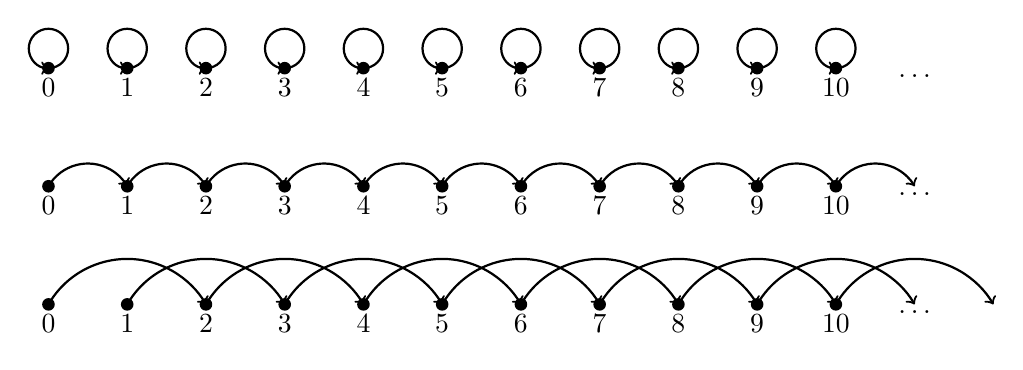
\begin{tikzpicture}
\def\paramVSep{-1.5}
\def\paramHSep{1}
\def\nPoints{10}
\def\rPoint{0.08}
\def\labelSep{0.1}
\foreach \i in {0, ..., \nPoints} {
    \fill (\i*\paramHSep, 0) circle[radius=\rPoint] node[below=\labelSep] {$\i$};
    \draw[thick, ->] (\i*\paramHSep, 0) arc (-90:270:{0.25*\paramHSep});
}
\node at (\paramHSep*\nPoints+\paramHSep, -\labelSep) {$\dots$};
\foreach \i in {0, ..., \nPoints} {
    \fill (\i*\paramHSep, \paramVSep) circle[radius=\rPoint] node[below=\labelSep] {$\i$};
    \draw[thick, ->] (\i*\paramHSep, \paramVSep) arc (150:30:{0.5*\paramHSep/sin(60)});
}
\node at (\paramHSep*\nPoints+\paramHSep, \paramVSep-\labelSep) {$\dots$};
\foreach \i in {0, ..., \nPoints} {
    \fill (\i*\paramHSep, 2*\paramVSep) circle[radius=\rPoint] node[below=\labelSep] {$\i$};
    \draw[thick, ->] (\i*\paramHSep, 2*\paramVSep) arc (150:30:{\paramHSep/sin(60)});
}
\node at (\paramHSep*\nPoints+\paramHSep, 2*\paramVSep-\labelSep) {$\dots$};
\end{tikzpicture}
\caption{Illustration de bijections de $\mathbb{N}$ vers quelques-uns de ses sous-ensembles : la fonction identité sur $\mathbb{N}$ et les fonctions $f_1: \mathbb{N} \to \mathbb{N^*}$ et $f_2: \mathbb{N} \to \mathbb{N} \setminus \lbrace 0, 1 \rbrace$ définies par : pour tout entier naturel $x$, $f_1(x) = x + 1$ et $f_2(x) = x + 2$.}
\label{fig:bij_N_N2}
\end{figure}

\subsubsection{Multiplication}
\label{subsub:multiplication}

\noindent\textbf{Définition de la multiplication :} Soit $E$ l'ensemble des fonctions de $\mathbb{N}$ dans $\mathbb{N}$. 
    On définit la suite $\mathrm{Mul}$ d'éléments de $E$ par récurrence de la manière suivante : 
    \begin{itemize}[nosep]
        \item Pour tout élément $m$ de $\mathbb{N}$, $\mathrm{Mul}(0)(m) = 0$.
        \item Pour tout élément $n$ de $\mathbb{N}$, pour tout élément $m$ de $\mathbb{N}$, $\mathrm{Mul}(n+1)(m) = \mathrm{Mul}(n)(m) + m$.
    \end{itemize}
    Notons que, pour tout élément $m$ de $\mathbb{N}$, on a $\mathrm{Mul}(1)(m) = m$. 
    Dans la suite, si $m$ et $n$ sont deux éléments de $\mathbb{N}$, on notera $m \times n$ l'entier $\mathrm{Mul}(n)(m)$. 
    Pour tous éléments $n$ et $m$ de $\mathbb{N}$, on a donc $m \times 0 = 0$, $m \times 1 = m$ et $m \times (n+1) = (m \times n) + m$.
    
    La multiplication est prioritaire sur l'addition. 
    Par exemple, si $a$, $b$ et $c$ sont trois éléments de $\mathbb{N}$, $a \times b + c$ est équivalent à $(a \times b) + c$ et $a + b \times c$ à $a + (b \times c)$.
    Le symbole $\times$ est parfois omis quand il n'y a pas de confusion possible. 
    Ainsi, si $n$ et $m$ sont deux entiers naturels, $n \times m$ pourra s'écrire $n m$.
    \index{Multiplication} \sindex[isy]{$\times$}

\medskip

\noindent\textbf{Lemme :} Pour tout entier naturel $n$, on a $0 \times n = 0$.

\medskip

\noindent\textbf{Démonstration :} On procède par récurrence sur $n$. 
    Puisque $0$ est un entier naturel et par définition de la multiplication, $0 \times 0 = 0$. 
    Donc, le résultat attendu est vrai pour $n = 0$. 
    Soit $n$ un entier naturel tel que $0 \times n = 0$. 
    Alors, $0 \times (n+1) = 0 + 0$.
    Puisque $0 + 0 = 0$, on en déduit $0 \times (n+1) = 0$. 
    Par récurrence, le résultat attendu est donc vrai pour tout entier naturel. 

   \done 

\medskip

\noindent\textbf{Lemme :} Pour tous entiers naturels $n$ et $m$, on a $(m+1) \times n = (m \times n) + n$.

\medskip

\noindent\textbf{Démonstration :} On procède par récurrence sur $n$. 
    Soit $P$ le prédicat à un paramètre défini par : $P(n): \forall m \in \mathbb{N}, \, (m+1) \times n = (m \times n) + n$. 
    Pour tout entier naturel $m$, on a $(m+1) \times 0 = 0$ et $(m \times 0) + 0 = 0 + 0 = 0$. 
    Donc, $P(0)$ est vrai. 

    Soit $n$ un entier naturel tel que $P(n)$ est vrai. 
    Soit $m$ un entier naturel. 
    Par définition de la multiplication, $(m+1) \times (n+1) = ((m+1) \times n) + (m+1)$. 
    Puisque $P(n)$ est vrai, cela donne $(m+1) \times (n+1) = ((m \times n) + n) + (m+1)$. 
    En utilisant deux fois l'associativté et la commutativité de l'addition, cela donne $(m+1) \times (n+1) = ((m \times n) + m) + (n+1)$. 
    Utilisant à nouveau la définition de la multiplication, cela se récrit en : $(m+1) \times (n+1) = (m \times (n+1)) + (n+1)$. 
    Cela étant vrai pour tout élémnt $m$ de $\mathbb{N}$, on en déduit que $P(n+1)$ est vrai. 

    Par récurrence, $P(n)$ est donc vrai pour tout entier naturel $n$, ce qui prouve le lemme.

   \done 

\medskip

\noindent\textbf{Lemme :} La multiplication est commutative : pour tous entiers naturels $n$ et $m$, on a $m \times n = n \times m$.

\medskip

\noindent\textbf{Démonstration :} On procède par récurrence sur $n$. 
    Soit $P$ le prédicat à un paramètre défini par : $P(n): \forall m \in \mathbb{N}, \, m \times n = n \times m$. 
    Pour tout entier naturel $m$, on a $m \times 0 = 0$ et $0 \times m = 0$. 
    Donc, $P(0)$ est vrai. 

    Soit $n$ un entier naturel tel que $P(n)$ est vrai. 
    Soit $m$ un entier naturel. 
    On a : $m \times (n+1) = (m \times n) + m$. 
    Puisque $P(n)$ est vrai, $m \times n = n \times m$. 
    Donc, $m \times (n+1) = (n \times m) + m$. 
    En utilisant le lemme précédent, il vient : $m \times (n+1) = (n+1) \times m$. 
    On en déduit que $P(n+1)$ est vrai. 

    Par récurrence, $P(n)$ est donc vrai pour tout entier naturel $n$. 

   \done 

\medskip

\noindent\textbf{Corolaire :} Pour tout entier naturel $n$, $1 \times n = n \times 1 = n$. 

\medskip

\noindent\textbf{Corolaire :} Pour tous entiers naturels $n$ et $m$, $(n+1) \times m = m \times (n+1) = (m \times n) + m = (n \times m) + m$. 

\medskip

\noindent\textbf{Lemme :} La multiplication est distributive sur l'addition : pour tous entiers naturels $n$, $m$ et $k$, on a $n \times (m + k) = (n \times m) + (n \times k)$.
    (Puisque la multiplication est commutative, on en déduit que, pour tous entiers naturels $n$, $m$ et $k$, on a $(m + k) \times n = (m \times n) + (k \times n)$.)

\medskip

\noindent\textbf{Démonstration :} On procède par récurrence sur $n$. 
    Soit $P$ le prédicat à un paramètre libre défini par : $P(n): \forall m \in \mathbb{N}, \, \forall k \in \mathbb{N}, \, n \times (m + k) = (n \times m) + (n \times k)$.

    Soit $m$ et $k$ deux entiers naturels. 
    On a : $0 \times (m+k) = 0$ et $(0 \times m) + (0 \times k) = 0 + 0 = 0$. 
    Donc, $0 \times (m+k) = (0 \times m) + (0 \times k)$. 
    Donc, $P(0)$ est vrai. 

    Soit $n$ un entier naturel et supposons que $P(n)$ est vrai. 
    Soit $m$ et $k$ deux enters naturels. 
    Alors, $(n+1) \times (m + k) = (n \times (m + k)) + (m + k)$. 
    Donc, puisque $P(n)$ est vrai, $(n+1) \times (m + k) = ((n \times m) + (n \times k)) + (m + k)$. 
    Puisque l'addition est associative et commutative, cela implique $(n+1) \times (m + k) = ((n \times m) + m) + ((n \times k) + k)$. 
    Donc, $(n+1) \times (m + k) = ((n+1) \times m) + ((n+1) \times k)$. 
    Donc, $P(n+1)$ est vrai. 

    Par récurrence, on en déduit que $P(n)$ est vrai pour tout entier naturel $n$, et donc le lemme.

   \done 

\medskip

\noindent\textbf{Lemme :} La multiplication est associative : pour tous entiers naturels $n$, $m$ et $k$, on a $n \times (m \times k) = (n \times m) \times k$.

\medskip

\noindent\textbf{Démonstration :} On procède par récurrence sur $n$. 
    Soit $P$ le prédicat à un paramètre libre défini par : $P(n): \forall m \in \mathbb{N}, \, \forall k \in \mathbb{N}, \, n \times (m \times k) = (n \times m) \times k$.

    Soit $m$ et $k$ deux entiers naturels. 
    On a : $0 \times (m \times k) = 0$ et $(0 \times m) \times k = 0 \times k = 0$. 
    Donc, $0 \times (m \times k) = (0 \times m) \times k$. 
    On en déduit que $P(0)$ est vrai. 
    Soit $n$ un entier naturel et supposons que $P(n)$ est vrai. 
    Soit $m$ et $k$ deux enters naturels. 
    Alors, $(n+1) \times (m \times k) = (n \times (m \times k)) + (m \times k)$. 
    Puisque $P(n)$ est vrai, cela donne $(n+1) \times (m \times k) = ((n \times m) \times k) + (m \times k)$. 
    En utilisant la distributivité de la multiplication sur l'addition, ceci devient : $(n+1) \times (m \times k) = ((n \times m) + m) \times k$, et donc $(n+1) \times (m \times k) = ((n + 1) \times m) \times k$.
    On en déduit que $P(n+1)$ est vrai. 
    
    Par récurrence, on en déduit que $P(n)$ est vrai pour tout entier naturel $n$, et donc le lemme.

   \done 

\medskip

\noindent\textbf{Lemme :} Soit $n$, $m$ et $k$ trois entiers naturels. Si $n \neq 0$ et $m > k$, alors $n \times m > n \times k$.

\medskip

\noindent\textbf{Démonstration :} On procède par récurrence sur $n$. 
    Soit $P$ le prédicat à un paramètre défini par : $P(n): n \neq 0 \Rightarrow \forall m \in \mathbb{N}, \, \forall k \in \mathbb{N}, \, m > k \Rightarrow n \times m > n \times k$. 
    Puisque $0 \neq 0$ est fausse, $P(0)$ est vrai. 

    Soit $n$ un entier naturel tel que $P(n)$ est vrai. 
    Si $n = 0$, $n+1 = 1$ ; alors, soit $m$ et $k$ deux entiers naturels tels que $m > k$, puisque $n m = m$ et $n k = k$, on a $n m > n k$, donc $P(n+1)$ est vrai. 
    Supposons maintenant $n \neq 0$. 
    Soit $m$ et $k$ deux entiers naturels tels que $m > k$. 
    Alors, $n m > n k$.
    Donc, $n m + k > n k + k$. 
    Puisque $m > k$, on a $m \geq k$, donc $k \leq m$, donc, on peut choisir un élément $q$ de $\mathbb{N}$ tel que $m = k + q$.
    Puisque $n m + k + q \geq n m + k$, on en déduit $n m + m > n k + k$.
    Donc, $(n+1) m > (n+1) k$. 
    Cela montre que $P(n) \Rightarrow P(n+1)$ pour tout entier naturel $n$. 

    Par récurrence, on en déduit que $P(n)$ est vrai pour tout entier naturel $n$, et donc le lemme.

   \done 

\medskip

\noindent\textbf{Corolaire :} Soit $n$, $m$ et $k$ trois entiers naturels tels que $m > k$. 
                               Alors $n \times m \geq n \times k$.

\medskip

\noindent\textbf{Démonstration :} Si $n \neq 0$, on a $n \times m > n \times k$ d'après le lemme, et donc $n \times m \geq n \times k$.
    Si $n = 0$, on a $n \times m = n \times k= 0$, et donc $n \times m \geq n \times k$. 
    Le résultat attendu est donc vrai dans les deux cas.

   \done 

\medskip

\noindent\textbf{Corolaire :} Soit $n$ et $m$ deux entiers naturels tels que $n \times m = 0$. Alors $n = 0$ ou $m = 0$. 

\medskip

\noindent\textbf{Démonstration :} Supposons par l'absurde $n \neq 0$ et $m \neq 0$.
    Alors, $m > 0$, donc, d'après le lemme précédent, $n \times m > n \times 0$, donc $n \times m > 0$, ce qui contredit l'énoncé.

   \done 

\medskip

\noindent\textbf{Corolaire :} Soit $a$, $b$, $c$ et $d$ quatre entiers naturels tels que $a > c$ et $b > d$. 
    Alors $a b > c d$.

\medskip

\noindent\textbf{Démonstration :} Puisque $a > c$, $a > 0$.
    Donc, puisque $b > d$, $a \times b > a \times d$. 
    En outre, puisque $a > c$, $a \times d \geq c \times d$.
    Donc, $a \times b > c \times d$.

   \done 

\medskip

\noindent\textbf{Corolaire :} Soit $n$, $m$ et $k$ trois entiers naturels tels que $n \neq 0$ et $n \times m = n \times k$. 
    Alors $m = k$.

\medskip

\noindent\textbf{Démonstration :} On ne peut avoir $m > k$ car cela impliquerait $n m > n k$, donc $m \leq k$.
   De même, ne peut avoir $k > m$ car cela impliquerait $n k > n m$ ; donc $k \leq m$. 
   On en déduit que $m = k$.

  \done 

\medskip

\noindent\textbf{Corolaire :} Soit $n$ et $m$ deux entiers naturels tels que $n > 1$ et $m > 0$. 
    Alors $n \times m > m$.

\medskip

\noindent\textbf{Démonstration :} Puisque $m > 0$ et $n > 1$, $m \times n > m \times 1$, ce qui donne $n \times m > m$.

   \done 

\medskip

\noindent\textbf{Corolaire :} Soit $n$ et $m$ deux entiers naturels tels que $n \geq 1$. 
    Alors $n \times m \geq m$.

\medskip

\noindent\textbf{Démonstration :} 
    Si $m = 0$, on a $n \times m = 0$, donc $n \times m = m$.
    Si $n = 1$, on a $n \times m = m$.
    Si aucune de ces conditions n'est satisfaite, $m > 0$ et $n > 1$, donc, d'après le corolaire précédent, $n \times m > m$.
    Dans tous les cas, on a bien $n \times m \geq m$.

   \done 

\medskip

\noindent\textbf{Définition (factoriel d'un entier naturel) :} On définit par récurrence le factoriel d'un entier naturel, noté par un point d'exclamation à sa droite, de la manière suivante%
\footnote{
    Il s'agit bien d'une définition par récurrence, obtenue en prenant (avec les notations du lemme de la section~\ref{subsub:suites}) $E = \mathbb{N}$, $e_0 = 1$ et pour $f$ la fonction de $\mathbb{N} \times \mathbb{N}$ vers $\mathbb{N}$ définie par : $\forall x \in \mathbb{N} \, \forall y \in \mathbb{N} \, f(x,y) = y \times (x+1)$.
}~:
\begin{itemize}[nosep]
    \item On pose $0! = 1$.
    \item Pour tout entier naturel $n$, on pose $(n+1)! = (n!) \times (n+1)$.
\end{itemize}
Le factoriel est prioritaire sur la multiplication et sur l'addition. 
\index{Factoriel}

\medskip

\noindent\textbf{Lemme :} Soit $n$, $m$ et $k$ trois entiers naturels tels que $m \geq k$.
    Alors, $n (m - k) = n m - n k$.

\medskip

\noindent\textbf{Démonstration :} 
    Tout d'abord, puisque $m \geq k$, $n m \geq m k$, donc $n m - n k$ existe.

    Montrons l'égalité par récurrence sur $n$. 
    Soit $P$ le prédicat à un paramètre libre définit par : $P(n): \forall m \in \mathbb{N} \, \forall k \in \mathbb{N} \, m \geq k \Rightarrow n (m-k) = n m - n k$. 
    
    Soit $m$ et $k$ deux entiers naturels tels que $m \geq k$.
    On a $0 \times (m-k) = 0$ et $0 \times m + 0 \times = 0 + 0 = 0$.
    Donc, $P(0)$ est vrai.

    Soit $n$ un enitier naturel tel que $P(n)$ est vrai. 
    Soit $m$ et $k$ deux entiers naturels tels que $m \geq k$. 
    Alors, $(n+1) (m-k) = n (m-k) + (m-k)$. 
    Puisque $P(n)$ est vrai, il vient : $(n+1)(m-k) = (n m - n k) + (m-k)$.
    Donc, $(n+1)(m-k) + (n+1) k = (n m - n k) + (m-k) + (n+1) k = (n m - n k) + (m-k) + n k + k = (n m - n k) + n k + (m-k) + k = n m + m = (n+1) m$.
    Donc, $(n+1)(m-k) = (n+1)m - (n+1) k$.
    On en déduit que $P(n+1)$ est vrai. 

    Par récurrence, $P(n)$ est donc vrai pour tout élément $n$ de $\mathbb{N}$, ce qui prouve le lemme.

    \done

\subsubsection{Puissance}
\label{subsub:puissance}

\noindent\textbf{Puissance d'entiers naturels :} Soit $E$ l'ensemble des fonctions de $\mathbb{N}$ dans $\mathbb{N}$. 
    On définit la suite $\mathrm{Exp}$ d'éléments de $E$ par récurrence de la manière suivante : 
    \begin{itemize}[nosep]
        \item Pour tout élément $m$ de $\mathbb{N}$, $\mathrm{Exp}(0)(m) = 1$.
        \item Pour tout élément $n$ de $\mathbb{N}$, pour tout élément $m$ de $\mathbb{N}$, $\mathrm{Exp}(n+1)(m) = \mathrm{Exp}(n)(m) \times m$.
    \end{itemize}
    Notons que, pour tout élément $m$ de $\mathbb{N}$, on a $\mathrm{Exp}(1)(m) = m$. 
    Dans la suite, pour tous éléments $n$ et $m$ de $\mathbb{N}$, on notera l'entier $\mathrm{Exp}(n)(m)$ par $m^n$. 
    Pour touts éléments $n$ et $m$ de $\mathbb{N}$, on a donc $m^0=1$, $m^1 = m$ et $m^{n+1} = m^n \times m$. 
    L'exponentiation est prioritaire sur la multiplication et l'addition. 
    Par exemple, si $a$, $b$ et $c$ sont trois éléments de $\mathbb{N}$, $a^b \times c$ est équivalent à $(a^b) \times c$ et $a^b + c$ est équivalent à $(a^b) + c$.
    \index{Puissance}

\medskip

\noindent\textbf{Lemme :} Pour tout entier naturel $n$, $1^n = 1$.

\medskip

\noindent\textbf{Démonstration :} On procède par récurrence sur $n$. 
    Pour $n = 0$, le résultat est vrai par définition de la puissance.
    Soit $m$ un entier naturel tel que $1^m = 1$. 
    Alors $1^{m+1} = 1^m \times 1 = 1 \times 1 = 1$. 
    Le résultat est donc vrai pour $n = m+1$. 
    Par récurrence, on en déduit qu'il est vrai pour tout entier naturel $n$.

   \done 

\medskip

\noindent\textbf{Lemme :} Pour tout entier naturel $n$, $0^{n+1} = 0$. 

\medskip

\noindent\textbf{Démonstration :} Soit $n$ un entier naturel. 
    On a : $0^{n+1} = 0^n \times 0$. 
    Puisque $0^n$ est un entier naturel, $0^n \times 0 = 0$. 
    Donc, $0^{n+1} = 0$.

   \done 
\medskip

\noindent\textbf{Corolaire :} 
    Soit $n$ un entier naturel tel que $n \neq 0$. 
    Alors, $n > 0$, donc $n - 1$ existe et est un entier naturel.
    Soit $m = n - 1$. 
    On a : $0^n = 0^{m + 1}$. 
    Donc, $0^n = 0$.

\medskip

\noindent\textbf{Lemme :} Soit $n$ et $m$ deux entiers naturels tels que $m \neq 0$. 
    Alors $m^n \neq 0$.

\medskip

\noindent\textbf{Démonstration :} On procède par récurrence qur $n$. 
    Pour $n = 0$, le résultat est évident car $m^0 = 1$. 
    Supposons le résultat vrai pour un entier naturel $n$. 
    Alors, $m^{n+1} = m^n \times m$. 
    Puisque $m^n \neq 0$ et $m \neq 0$, $m^{n+1} \neq 0$. 
    Par récurrence, on en déduit le lemme.

   \done 

\medskip

\noindent\textbf{Lemme :} Soit $n$, $m$ et $p$ trois entiers naturels. 
    Alors, $p^{n+m} = p^n \times p^m$.

\medskip

\noindent\textbf{Démonstration :} On procède par récurrence sur $n$. 
    Soit $P$ le prédicat à un paramètre libre défini par : $P(n): \forall p \in \mathbb{N}, \forall m \in \mathbb{N}, \, p^{n+m} = p^n \times p^m$. 
    Soit $p$ et $m$ deux entiers naturels. 
    Puisque $0 + m = m$, on a $p^{0 + m} = p^m$. 
    Par ailleurs, puisque $p^0 = 1$, $p^0 \times p^m = p^m$. 
    Donc, $p^{0+m} = p^0 \times p^m$. 
    Cela montre que $P(0)$ est vrai. 

    Soit $n$ un entier naturel tel que $P(n)$ est vrai. 
    On veut montrer que $P(n+1)$ est vrai. 
    Soit $m$ et $p$ deux entiers naturels. 
    Par commutativité et transitivité de l'addition, on a : $p^{m+(n+1)} = p^{m+(1+n)} = p^{(m+1)+n}$. 
    Puisque $P(n)$ est vrai, on en déduit que $p^{m+(n+1)} = p^{m+1} \times p^n$. 
    Par définition de la puissance d'entiers, cela donne $p^{m+(n+1)} = (p^m \times p) \times p^n$. 
    En utilisant l'associativité et la commutativité de la multiplication, il vient : $p^{m+(n+1)} = p^m \times (p^n \times p)$. 
    Enfin, utiliser à nouveau la définition de la puissance d'entiers donne : $p^{m+(n+1)} = p^m \times p^{n+1}$. 
    Cela montre que $P(n+1)$ est vrai. 
    Par récurrence, le prédicat $P(n)$ est donc vrai pour tout entier naturel $n$, ce qui prouve le lemme. 

   \done 

\medskip

\noindent\textbf{Lemme :} Soit $n$, $m$ et $p$ trois entiers naturels tels que $m > p$. 
    Alors, $m^{n+1} > p^{n+1}$. 

\medskip

\noindent\textbf{Démonstration :} On procède par récurrence sur $n$. 
    Soit $P$ le prédicat à un paramètre défini par : $P(n): \forall m \in \mathbb{N}, \forall p \in \mathbb{N}, m > p \Rightarrow m^{n+1} > p^{n+1}$. 
    Soit $m$ et $p$ deux entiers naturels tels que $m > p$. 
    On a $m^{0+1} = m^1 = m$ et $p^{0+1} = p^1 = p$. 
    Donc, $m^{0+1} > p^{0+1}$. 
    On en déduit que $P(0)$ est vrai.

    Soit $n$ un entier naturel tel que $P(n)$ est vrai. 
    Soit $m$ et $p$ deux entiers naturels tels que $m > p$. 
    On a $m^{(n+1)+1} = m^{n+1} \times m$ et $p^{(n+1)+1} = p^{n+1} \times p$. 
    Puisque $P(n)$ est vrai, on a $m^{n+1} > p^{n+1}$. 
    Donc, $m^{(n+1)+1} > p^{n+1} \times m$. 
    Puisque $m > p$, $p^{n+1} \times m \geq p^{n+1} \times p$, et donc $p^{n+1} \times m \geq p^{(n+1)+1}$. 
    Donc, $m^{(n+1)+1} > p^{(n+1)+1}$. 
    On en déduit que $P(n+1)$ est vrai. 

    Par récurrence, $P(n)$ est donc vrai pour tout entier naturel $n$, ce qui prouve le lemme.

   \done 

\medskip

\noindent\textbf{Corolaire :} 
    Soit $n$ un entier naturel tel que $n \neq 0$. 
    Alors, $n > 0$, donc $n - 1$ existe et est un entier naturel.
    Soit $q = n - 1$. 
    Soit $m$ et $p$ deux entiers naturels tels que $m > p$.
    Alors, $m^n = m^{q+1}$ et $p^n = p^{q+1}$. 
    D'après le lemme précédent, on en déduit $m^n > p^n$. 

\medskip

\noindent\textbf{Corolaire :} 
    Soit $m$ et $p$ deux entiers naturels tels que $m \geq p$.
    Par définition de la puissance, $m^0 = p^0 = 1$.
    En outre, si $m = p$, alors $m^n = p^n$ pour tout entier naturel $n$ et, si $m > p$, $m^n > p^n$ pour tout entier naturel $n$ distinct de $0$ d'après le corolaire précédent.
    On en déduit que, pour tout entier naturel $n$, $m^n \geq p^n$.

\medskip

\noindent\textbf{Lemme :} Soit $n$, $m$ et $p$ trois entiers naturels tels que $m > p$. 
    Alors, si $n > 1$, $n^m > n^p$. 
    (Rappelons que l'on a : $1^m = 1^p = 1$.)

\medskip

\noindent\textbf{Démonstration :} On procède par récurrence sur $m$. 
    Soit $P$ le prédicat à un paramètre défini par : $P(m): \forall n \in \mathbb{N}, \forall p \in \mathbb{N}, (m > p) \wedge (n > 1) \Rightarrow n^m > n^p$. 
    Pour $m=0$, il n'existe aucun entier naturel $p$ tel que $m > p$, donc $P(0)$ est vrai. 

    Soit $m$ un entier naturel tel que $P(m)$ est vrai. 
    Soit $n$ et $p$ deux entiers naturels tels que $m+1 > p$ et $n > 1$. 
    Alors, $p = m$ ou $p < m$. 
    Dans le second cas, puisque $P(m)$ est vrai, on a $n^m > n^p$. 
    Donc, dans les deux cas, $n^m \geq n^p$. 
    En outre, $n \neq 0$, donc $n^m \neq 0$.
    Puisque $n > 1$ et $n^{m+1} = n^m \times n$, on en déduit que $n^{m+1} > n^m$, et donc $n^{m+1} > n^p$. 
    Donc, $P(m+1)$ est vrai. 

    Par récurrence, $P(m)$ est donc vrai pour tout entier naturel $m$.

   \done 


\subsubsection{Puissances de fonctions}

Soit $E$ un ensemble et $f$ une fonction de $E$ vers $E$. 
On définit les puissances de $f$, $f^n$, pour $n \in \mathbb{N}$ de la manière suivante :
\begin{itemize}[nosep]
    \item $f^0$ est la fonction identité, qui à tout élément $x$ de $E$ associe $x$. 
    \item Pour tout élément $n$ de $\mathbb{N}$, $f^{n+1} = f \circ f^n$. 
        (Cela définit bien une fonction de $E$ vers $E$, commecomposée de deux fonctions de $E$ vers $E$.)
\end{itemize}
(Il s'agit d'une définition par récurrence d'une suite de fonctions de $E$ vers $E$.) 
Notons que, pour tout entier naturel $n$ tel que $n \neq 0$, on a $f^{n} = f \circ f^{n-1}$ (puisque n = (n-1) + 1).
Notons aussi que $f^1 = f$. 
La puissance est prioritaire sur $\circ$.
\index{Puissance}

\medskip

\noindent\textbf{Lemme :} 
    Soit $E$ un ensemble et $f$ une fonction de $E$ vers $E$.
    Soit $n$ un entier naturel. 
    Alors, $f^n \circ f = f^{n+1}$.

\medskip

\noindent\textbf{Démonstration :} On procède par récurrence sur $n$. 
    Soit $P$ le prédicat à un paramètre libre défini par : $P(n): f^n \circ f = f^{n+1}$.
    Les deux fonctions $(f^0) \circ f$ et $f^1$ sont deux fonctions de $E$ dans $E$ (la première, comme composée de fonctions de $E$ dans $E$). 
    Soit $x$ un élément de $E$. 
    On a : $(f^0 \circ f)(x) = f^0(f(x)) = f(x) = f^1(x)$. 
    Donc, $f^0 \circ f = f^1$.
    Donc, et puisque $1 = 0+1$, $P(0)$ est vrai. 
    
    Soit $n$ un entier naturel tel que $P(n)$ est vrai. 
    Les deux fonctions $(f^{n+1}) \circ f$ et $f^{(n+1)+1}$ sont deux fonctions de $E$ dans $E$ (la première, comme composée de fonctions de $E$ dans $E$). 
    En outre, on a $f^{(n+1)+1} = f \circ f^{n+1}$.
    Puisque $P(n)$ est vrai, cela donne $f^{(n+1)+1} = f \circ (f^n \circ f)$. 
    Puisque la composition de fonctions est associative, cela donne : $f^{(n+1)+1} = (f \circ f^n) \circ f$.
    Enfin, en utilisant la définition de la puissance de fonction, il vient : $f^{(n+1)+1} = f^{n+1} \circ f$.
    Cela montre que $P(n+1)$ est vrai.
    
    Par récurrence, on conclut que $P(n)$ est vrai pour tout entier naturel $n$, ce qui prouve le lemme. 

   \done 

\medskip

\noindent\textbf{Lemme :} 
    Soit $E$ un ensemble et $f$ une fonction de $E$ vers $E$.
    Soit $n$ et $m$ deux entiers naturels. 
    Alors, $f^{n+m} = (f^n) \circ (f^m)$.

\medskip

\noindent\textbf{Démonstration :} \textit{(La démonstration est essentiellement identique à celle donnée pour la puissance d'entiers, en utilisant l'associativité de $\circ$ et le résultat ci-dessus en guise de commutativité. Nous la donnons ici explicitement afin d'être complets.)}

    On procède par récurrence sur $n$. 
    Soit $P$ le prédicat à un paramètre libre défini par : $P(n) : \forall m \in \mathbb{N}, \, f^{n+m} = f^n \circ f^m$. 
    Puisque $f^0$ est la fonction identité, on a $f^0 \circ f^m = f^m$ pour tout entier naturel $m$. 
    Puisque $0 + m = m$ pour tout entier naturel $m$, on en déduit que $P(0)$ est vrai. 

    Soit $n$ un entier naturel tel que $P(n)$ est vrai. 
    Soit $m$ un entier naturel. 
    On a d'après le lemme précédent : $f^{n+1} \circ f^m = (f^n \circ f) \circ f^m$. 
    En utilisant l'associativité de $\circ$, il vient : $f^{n+1} \circ f^m = f^n \circ (f \circ f^m)$. 
    La définition de la puissance de fonction donne alors : $f^{n+1} \circ f^m = f^n \circ f^{m+1}$. 
    Puisque $P(n)$ est vrai, cela donne : $f^{n+1} \circ f^m = f^{n+(m+1)}$. 
    Enfin, en utilisant la commutativité et l'associativité de l'addition, il vient : $f^{n+1} \circ f^m = f^{(n+1)+m}$. 
    On en déduit que $P(n+1)$ est vrai. 

    Par récurrence, on conclut que $P(n)$ pour tout entier naturel $n$, et donc le lemme.

   \done 

\medskip

\noindent\textbf{Lemme :} 
    Soit $E$ un ensemble et $f$ une fonction de $E$ vers $E$.
    Soit $n$ et $m$ deux entiers naturels. 
    Alors, $f^n \circ f^m = f^m \circ f^n$.

\medskip

\noindent\textbf{Démonstration :}%
    \footnote{La démonstration est évidente en utilisant le lemme précédent et la commutativité de l'addition : en admettant ces éléments, on a $f^n \circ f^m = f^{n+m} = f^{m+n} = f^m \circ f^n$.
    Nous donnons ici unr démonstration alternative, plus pédestre.}
    On procède par récurrence sur $n$.
    Soit $P$ le prédicat à un paramètre libre défini par : $P(n): \forall m \in \mathbb{N}, \, f^n \circ f^m = f^m \circ f^n$. 
    Soit $m$ un entier naturel. 
    Puisque $f^0$ est la fonction identité sur $E$, on a $f^0 \circ f^m = f^m$ et $f^m \circ f^0 = f^m$.
    Donc, $f^0 \circ f^m = f^m \circ f^0$. 
    Cela étant vrai pour tout entier natiurel $m$, on en déduit que $P(0)$ est vrai.

    Soit $n$ un entier naturel tel que $P(n)$ est vrai. 
    Soit $m$ un entier naturel. 
    Les deux fonctions $f^{n+1} \circ f^m$ et $f^m \circ f^{n+1}$ sont les composées de deux fonctions de $E$ dans $E$. 
    Ce sont donc encore des fonctions de $E$ dans $E$. 
    On a : $f^{n+1} \circ f^m = (f^n \circ f) \circ f^m$.
    L'associativité de la composition de fonctions donne : $f^{n+1} \circ f^m = f^n \circ (f \circ f^m)$.
    En utilisant la définition de la puissance de fonction, il vient : $f^{n+1} \circ f^m = f^n \circ f^{m+1}$.
    Puisque $P(n)$ est vrai, cela donne : $f^{n+1} \circ f^m = f^m \circ f^{n+1}$. 
    Cela étant vrai pour tout élément $m$ de $\mathbb{N}$, on en déduit que $P(n+1)$ est vrai. 

    Par récurrence, on en déduit que $P(n)$ est vrai pour tout entier naturen $n$, ce qui prouve le lemme.

   \done 

\subsubsection{Puissances d'ensembles}

Soit $E$ un ensemble et $n$ un entier naturel. 
On note $E^n$ l'ensemble des fonctions de $n$ vers $E$. 
(Notons que cela est cohérent avec les notations définies section~\ref{sub:fonctions})
Soit $n$ éléments de $E$ notés $e_0$, $e_1$, ..., $e_{n-1}$. 
On note (quand il n'y a pas d'ambiguité avec d'autres notations) $\left( e_0, e_1, \dots e_{n-1} \right)$ la fonction $f$ de $n$ vers $E$ telle que $f(0) = e_0$, $f(1) = e_1$, ..., $f(n-1) = e_{n-1}$. 
Quand il n'y a pas d'ambiguité, si $f$ est une fonction de $n$ vers $E^{n}$ et $i$ un élément de $[\![1,n]\!]$, on note parfois $f_i$ l'élément $f(i-1)$ de $E$.
\index{Puissance}

Soit $n$ un entier naturel et $E$ un ensemble. 
Une fonction de $n$ vers $E$ est parfois appelée \textit{séquence de $n$ éléments de $E$} ou \textit{$n$-uplet d'éléments de $E$}.

\subsubsection{Produit cartésien de plusieurs ensembles}

Soit $n$ un entier naturel non nul et $E_1$, $E_2$, ..., $E_n$ des ensembles (où le dernier symbole est absent si $n \leq 2$ et le symbole $E_2$ est absent si $n = 1$). 
On note $E_1 \times E_2 \times \cdots \times E_n$ l'ensemble $( \cdots ( E_1 \times E_2 ) \times  \cdots ) \times E_n$.

Soit $e_1$ un élément de $E_1$, $E_2$ un élément de $E_2$, ..., $e_n$ un élément de $E_n$. 
L'élément $(( \cdots ( e_1, e_2 ), \dots ), e_n)$ pourra être noté $(e_1, e_2, \dots e_n)$ s'il n'y a pas d'ambiguité. 
